% ==============================================================================
% CHƯƠNG 5: PHÂN TÍCH DỮ LIỆU VÀ TRỰC QUAN HÓA
% ==============================================================================
\section{Phân tích dữ liệu và trực quan hóa}
\label{sec:phan_tich_truc_quan}

% ==============================================================================
% SUBSECTION 5.X: KHUNG CHUẨN CHO MỖI TAB (ÁP DỤNG TỪ TAB 01 ĐẾN TAB 05)
% ==============================================================================
\subsection{Mục tiêu 1: Bức tranh thị trường}
\label{subsec:tab1}

% ------------------------------------------------------------------------------
% 5.1.1 BỐI CẢNH VÀ MÔ HÌNH DỮ LIỆU CỦA TAB
% ------------------------------------------------------------------------------
\subsubsection{Bối cảnh phân tích và mô hình dữ liệu}
\label{subsubsec:tab1_schema}

\noindent\textbf{Bối cảnh và mục tiêu phân tích:}
Tab 1: ``Bức Tranh Thị Trường'' giữ vai trò nền tảng trong đồ án, cung cấp một góc nhìn toàn cảnh và đa chiều về quy mô, cơ cấu và các đặc trưng cốt lõi của thị trường xe ô tô (bao gồm cả xe cũ và xe mới) đang giao dịch tại Việt Nam. Phân tích này hướng tới việc làm rõ cán cân thị phần giữa các thương hiệu, sự ưa chuộng về kiểu dáng thân xe (body type), tính chất cung - cầu theo tình trạng (Mới/Cũ), nguồn gốc xuất xứ (Lắp ráp/Nhập khẩu) và chu kỳ tuổi đời phương tiện theo năm sản xuất. Qua đó, tab này đặt cơ sở thực chứng để trả lời câu hỏi tổng thể: ``Cấu trúc thị trường ô tô Việt Nam đang được định hình bởi những phân khúc, thương hiệu và chu kỳ sản phẩm nào?''.

{\small
\begin{xltabular}{\textwidth}{L{3cm} L{3.5cm} L{4cm} Y}
\caption{Các trường dữ liệu khai thác cho Tab 1}
\label{tab:schema_tab1} \\
\hline
\textbf{Tên cột} & \textbf{Bảng nguồn} & \textbf{Ý nghĩa dữ liệu} & \textbf{Phục vụ phân tích} \\ \hline
\endfirsthead

\multicolumn{4}{l}{\textit{Bảng \ref{tab:schema_tab2} (tiếp theo)}} \\
\hline
\textbf{Tên cột} & \textbf{Bảng nguồn} & \textbf{Ý nghĩa dữ liệu} & \textbf{Phục vụ phân tích} \\ \hline
\endhead

\hline
\multicolumn{4}{r}{\textit{Còn tiếp ở trang sau}} \\
\endfoot

\hline
\endlastfoot

Mã tin & fact\_car\_listings & Mã định danh duy nhất của mỗi tin đăng bán xe & Biến đo lường (Đếm tổng số lượng) \\
Giá (triệu VND) & fact\_car\_listings & Mức giá chào bán niêm yết của phương tiện & Biến đo lường (Tính giá trung vị) \\
Năm sản xuất & fact\_car\_listings & Tuổi đời của xe (từ 1990 đến 2025) & Trục thời gian / Chu kỳ sản phẩm \\
Tên hãng & dim\_brand & Thương hiệu sản xuất (Toyota, Hyundai, Ford...) & Phân loại / Treemap thị phần hãng xe \\
Tên dòng xe & dim\_body\_type & Kiểu dáng thân xe (SUV, Sedan, Crossover...) & Phân loại / Biểu đồ dòng xe phổ biến \\
Tình trạng & dim\_condition & Mức độ sử dụng phương tiện (Xe cũ vs Xe mới) & Phân loại / Donut chart cán cân cung cầu \\
Xuất xứ & dim\_origin & Nguồn gốc nguồn cung (Lắp ráp vs Nhập khẩu) & Phân loại / Donut chart nguồn gốc \\
\end{xltabular}
}


% ------------------------------------------------------------------------------
% 5.1.2 KHỐI CHỈ SỐ KPI TỔNG QUAN
% ------------------------------------------------------------------------------
\subsubsection{Khối chỉ số KPI tổng quan}
\label{subsubsec:tab1_kpi}

{\small
\begin{xltabular}{\textwidth}{L{3cm} L{2.5cm} L{4cm} Y}
\caption{Các chỉ số KPI điều hướng trên dashboard Tab 1}
\label{tab:kpi_tab1} \\
\hline
\textbf{Thẻ KPI} & \textbf{Giá trị ghi nhận} & \textbf{Công thức hoặc Logic} & \textbf{Ý nghĩa định hướng} \\ \hline
\endfirsthead

\multicolumn{4}{l}{\textit{Bảng \thetable{} (tiếp theo)}} \\
\hline
\textbf{Thẻ KPI} & \textbf{Giá trị ghi nhận} & \textbf{Công thức hoặc Logic} & \textbf{Ý nghĩa định hướng} \\ \hline
\endhead

\hline
\multicolumn{4}{r}{\textit{Còn tiếp ở trang sau}} \\
\endfoot

\hline
\endlastfoot

Tổng số tin đăng & 33.848 & Đếm tổng số dòng dữ liệu (\texttt{COUNT}) & Xác định quy mô tổng thể của mẫu dữ liệu, đảm bảo độ tin cậy và tính đại diện cho thị trường ô tô. \\
Tổng số hãng xe & 91 hãng & Đếm số thương hiệu duy nhất (\texttt{COUNT DISTINCT}) & Thể hiện mức độ đa dạng chủng loại và tính cạnh tranh gay gắt của các thương hiệu ô tô tại Việt Nam. \\
Giá trung vị toàn thị trường & 638 triệu VND & Lấy giá trị median của cột \texttt{Giá (triệu VND)} & Định vị ``mức giá trung tâm'' đại diện cho ngân sách mua xe phổ thông của đại đa số người tiêu dùng. \\
Năm SX phổ biến nhất & 2023 (4.006 xe) & Xác định yếu tố xuất hiện nhiều nhất (\texttt{MODE}) & Chỉ ra độ tuổi sản phẩm chiếm ưu thế trên thị trường thứ cấp (xe lướt từ 1-2 năm tuổi). \\
\end{xltabular}
}


% ------------------------------------------------------------------------------
% 5.1.3 CÂU HỎI SMART 1
% ------------------------------------------------------------------------------
\subsubsection{Câu hỏi 1}
\label{subsubsec:tab1_q1}

\noindent \textbf{Nội dung câu hỏi: Cơ cấu thị phần theo thương hiệu và kiểu dáng thân xe (dòng xe) trên thị trường ô tô Việt Nam phân hóa như thế nào, và những thương hiệu/dòng xe nào đang nắm giữ vị thế thống trị?}

% --- Biểu đồ 1.1 ---
\begin{figure}[H]
\centering
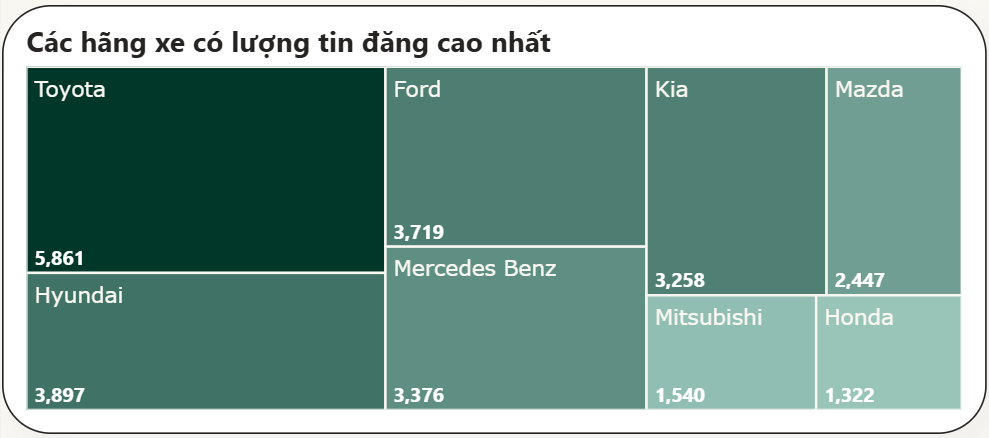
\includegraphics[width=0.8\textwidth]{graphics/Tab01/1.1.png}
\caption{Biểu đồ khối - Treemap Top các hãng xe theo số lượng tin đăng}
\label{fig:tab1_chart_1_1}
\end{figure}

\noindent\textbf{Loại biểu đồ:} Biểu đồ khối - Treemap.

\begin{itemize}
    \item \textbf{Mục đích và ý nghĩa:} Trực quan hóa thị phần tương quan của Top 15 thương hiệu ô tô lớn nhất, giúp người đọc lập tức nhận diện các thương hiệu chi phối thị trường thông qua tỷ lệ diện tích trực quan.
    
    \item \textbf{Sử dụng dữ liệu:}
    \begin{itemize}
        \item Bảng dữ liệu nguồn: \texttt{fact\_car\_listings} kết hợp \texttt{dim\_brand}.
        \item Chỉ số: Đếm số lượng \texttt{Mã tin} nhóm theo \texttt{Tên hãng} (lấy Top 15 thương hiệu hàng đầu).
    \end{itemize}
    
    \item \textbf{Thiết kế và giải thích:} Dạng biểu đồ Treemap phân bố không gian tối ưu cho dữ liệu có nhiều danh mục. Sử dụng một tông màu thuần (Xanh lục đậm) nhất quán để loại bỏ nhiễu thị giác, buộc mắt người xem tập trung trực tiếp vào quy mô diện tích khối.
    
    \item \textbf{Mã hóa trực quan:}
    \begin{itemize}
        \item Kích thước diện tích ô: Tỷ lệ thuận với số lượng tin đăng chào bán của từng hãng xe.
        \item Nhãn thông tin: Hiển thị tên hãng kèm theo số lượng xe và tỷ lệ phần trăm thị phần tương ứng.
    \end{itemize}
    
    \item \textbf{Nhận định và phân tích:}
    \begin{itemize}
        \item Thứ bậc và vị thế thống trị: Toyota vững vàng ở vị trí số 1 với 5.861 tin đăng (chiếm 17,32\% thị phần toàn thị trường), xếp tiếp theo là Hyundai với 3.897 xe (11,51\%) và Ford với 3.719 xe (10,99\%).
        \item Tỷ trọng nhóm dẫn đầu: Top 5 thương hiệu hàng đầu (Toyota, Hyundai, Ford, Mercedes-Benz với 3.376 xe - 9,97\%, và Kia với 3.258 xe - 9,63\%) hợp thành một tập đoàn thống trị chiếm tới 59,42\% tổng lượng xe giao dịch.
        \item Sự hiện diện thương hiệu sang và thương hiệu Việt: Mercedes-Benz là thương hiệu hạng sang duy nhất lọt vào Top 4 thị phần. VinFast - thương hiệu ô tô Việt Nam - đã ghi dấu ấn ở vị trí thứ 11 với 794 xe (chiếm 2,35\% thị phần).
    \end{itemize}
\end{itemize}

% --- Biểu đồ 1.2 ---
\begin{figure}[H]
\centering
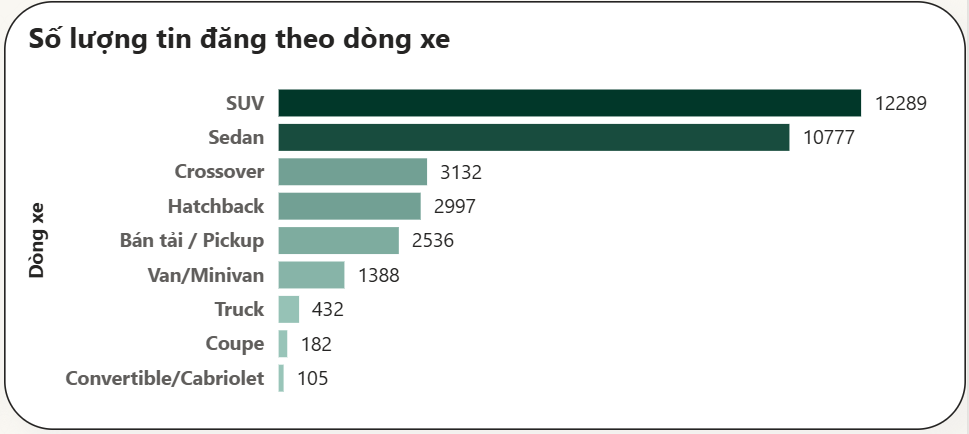
\includegraphics[width=0.8\textwidth]{graphics/Tab01/1.2.png}
\caption{Biểu đồ thanh ngang phân bố số lượng tin đăng theo dòng xe (kiểu dáng thân xe)}
\label{fig:tab1_chart_1_2}
\end{figure}

\noindent\textbf{Loại biểu đồ:} Biểu đồ thanh ngang - Horizontal Bar Chart.

\begin{itemize}
    \item \textbf{Mục đích và ý nghĩa:} Đo lường thị hiếu người tiêu dùng Việt Nam đối với các kiểu dáng thân xe (body type), từ đó xác định xu hướng thiết kế ô tô đang dẫn dắt thị trường.
    
    \item \textbf{Sử dụng dữ liệu:}
    \begin{itemize}
        \item Bảng dữ liệu nguồn: \texttt{fact\_car\_listings} kết hợp \texttt{dim\_body\_type}.
        \item Chỉ số: Đếm số lượng \texttt{Mã tin} nhóm theo \texttt{Tên dòng xe}, xếp hạng giảm dần.
    \end{itemize}
    
    \item \textbf{Thiết kế và giải thích:} Biểu đồ thanh ngang giúp dễ dàng đọc nhãn các kiểu dáng thân xe dài mà không bị che khuất. Các thanh được sắp xếp từ cao xuống thấp tạo cấu trúc trực quan rõ ràng.
    
    \item \textbf{Nhận định và phân tích:}
    \begin{itemize}
        \item Hai trụ cột thị trường: SUV và Sedan tạo thành hai phân khúc áp đảo tuyệt đối. SUV đứng đầu với 12.289 tin đăng (chiếm 36,31\%), theo sát là Sedan với 10.777 tin đăng (chiếm 31,84\%). Tổng cộng hai dòng xe này nắm giữ tới 68,15\% thị phần.
        \item Phân khúc đô thị và đa dụng: Crossover (3.132 xe - 9,25\%) và Hatchback (2.997 xe - 8,85\%) xếp các vị trí tiếp theo, phản ánh nhu cầu di chuyển linh hoạt trong đô thị. Bán tải / Pickup chiếm 2.536 xe (7,49\%) phục vụ nhóm khách hàng thích xe gầm cao cá tính hoặc kinh doanh thương mại.
    \end{itemize}
\end{itemize}

\noindent\textbf{Kết luận và đề xuất hành động cho câu hỏi 1:} 
\begin{itemize}
    \item \textbf{Đúc kết cốt lõi:} Thị trường ô tô Việt Nam có độ tập trung cao vào các thương hiệu phổ thông châu Á (Toyota, Hyundai, Kia) và xe gầm cao (SUV/Crossover) kết hợp Sedan truyền thống.
    \item \textbf{Đề xuất hành động:} 
    \begin{itemize}
        \item \textbf{Đối với đại lý kinh doanh xe:} Tối ưu kho hàng bằng việc tập trung 65 - 70\% nguồn vốn vào các dòng xe SUV và Sedan thuộc Top 5 hãng xe (Toyota, Hyundai, Ford, Kia, Mazda) nhằm đảm bảo tốc độ quay vòng vốn và thanh khoản nhanh nhất.
        \item \textbf{Đối với nhà phân phối / hãng xe mới:} Cần cân nhắc kỹ khi đầu tư vào các phân khúc ngách do thị phần cộng gộp dưới 1\%, thay vào đó nên tập trung vào dải sản phẩm SUV/Crossover cỡ B/C đang rất được ưa chuộng.
    \end{itemize}
\end{itemize}


% ------------------------------------------------------------------------------
% 5.1.4 CÂU HỎI SMART 2
% ------------------------------------------------------------------------------
\subsubsection{Câu hỏi 2}
\label{subsubsec:tab1_q2}

\noindent \textbf{Nội dung câu hỏi: Cấu trúc nguồn cung thị trường được phân bổ như thế nào theo tình trạng phương tiện (Xe cũ vs Xe mới), xuất xứ nguồn cung (Lắp ráp vs Nhập khẩu) và chu kỳ sản xuất (năm sản xuất)?}

% --- Biểu đồ 2.1 ---
\begin{figure}[H]
\centering
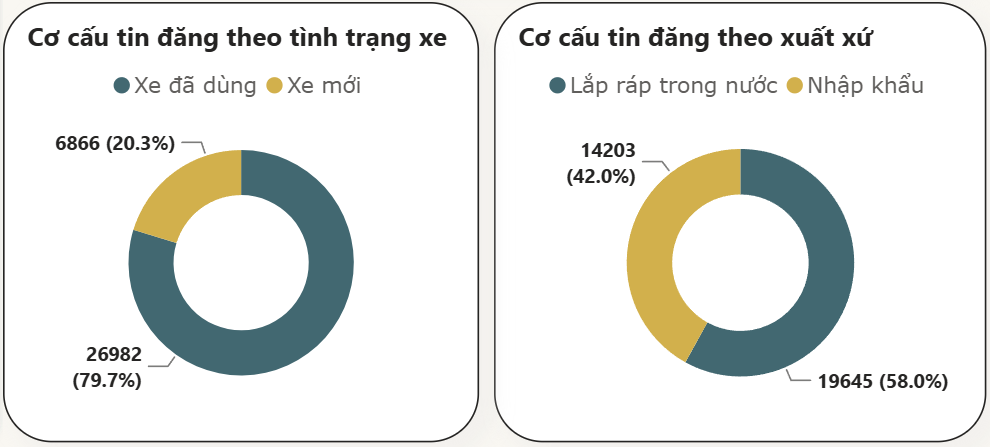
\includegraphics[width=0.8\textwidth]{graphics/Tab01/2.1.png}
\caption{Biểu đồ Donut kép biểu diễn tỷ lệ phân bổ theo Tình trạng và Xuất xứ}
\label{fig:tab1_chart_2_1}
\end{figure}

\noindent\textbf{Loại biểu đồ:} Biểu đồ Donut - Double Donut Charts.

\begin{itemize}
    \item \textbf{Mục đích và ý nghĩa:} So sánh cán cân tỷ lệ giữa xe đã qua sử dụng và xe mới, cũng như cán cân nguồn cung giữa xe lắp ráp trong nước (CKD) và xe nhập khẩu nguyên chiếc (CBU).
    
    \item \textbf{Sử dụng dữ liệu:}
    \begin{itemize}
        \item Bảng dữ liệu nguồn: \texttt{fact\_car\_listings} kết hợp \texttt{dim\_condition} và \texttt{dim\_origin}.
        \item Chỉ số: Tỷ lệ phần trăm tính theo đếm tổng số tin đăng cho các nhóm \texttt{Tình trạng} và \texttt{Xuất xứ}.
    \end{itemize}
    
    \item \textbf{Thiết kế và giải thích:} Biểu đồ Donut kép đặt cạnh nhau giúp người xem dễ dàng đối chiếu hai lát cắt nhị phân quan trọng của thị trường. Nhóm chi phối được phối màu xanh rêu, nhóm phụ phối màu vàng gold.
    
    \item \textbf{Nhận định và phân tích:}
    \begin{itemize}
        \item Về tình trạng xe: Xe đã qua sử dụng (xe cũ) chiếm tỷ trọng áp đảo 79,72\% (với 26.982 tin đăng), trong khi xe mới chỉ chiếm 20,28\% (6.866 tin đăng). Điều này khẳng định sàn giao dịch mang tính chất trọng tâm là thị trường xe cũ thứ cấp.
        \item Về xuất xứ nguồn cung: Xe lắp ráp trong nước (CKD) chiếm ưu thế với 58,04\% (19.645 tin đăng), xe nhập khẩu (CBU) chiếm 41,96\% (14.203 tin đăng). Cán cân này phản ánh năng lực lắp ráp nội địa ngày càng tăng nhờ các chính sách ưu đãi thuế phí của Chính phủ.
    \end{itemize}
\end{itemize}

% --- Biểu đồ 2.2 ---
\begin{figure}[H]
\centering
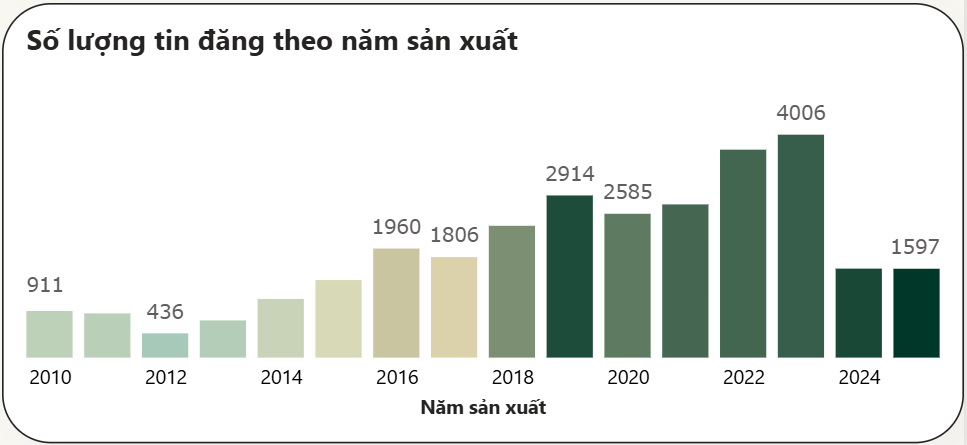
\includegraphics[width=0.8\textwidth]{graphics/Tab01/2.2.png}
\caption{Biểu đồ cột phân bố số lượng xe theo năm sản xuất (1990 - 2025)}
\label{fig:tab1_chart_2_2}
\end{figure}

\noindent\textbf{Loại biểu đồ:} Biểu đồ cột dọc - Column Chart.

\begin{itemize}
    \item \textbf{Mục đích và ý nghĩa:} Đánh giá phân bố tuổi đời xe, xác định chu kỳ thanh lý phổ biến và vùng tập trung mật độ giao dịch cao nhất trên thị trường ô tô.
    
    \item \textbf{Sử dụng dữ liệu:}
    \begin{itemize}
        \item Bảng dữ liệu nguồn: \texttt{fact\_car\_listings}.
        \item Chỉ số: Đếm số lượng xe nhóm theo \texttt{Năm sản xuất} từ 2010 đến 2025.
    \end{itemize}
    
    \item \textbf{Thiết kế và giải thích:} Trục hoành biểu diễn tiến trình thời gian tăng dần, giúp nhận diện rõ sự tích tụ dữ liệu theo chu kỳ sóng.
    
    \item \textbf{Nhận định và phân tích:}
    \begin{itemize}
        \item Vùng tập trung trọng điểm: Dữ liệu phân phối lệch trái mạnh về phía các năm gần đây. Nhóm xe sản xuất từ năm 2020 đến 2025 chiếm tới 48,09\% toàn thị trường (16.277 xe).
        \item Đỉnh sóng thanh lý: Năm sản xuất 2023 có lượng xe giao dịch cao nhất đạt 4.006 xe (11,84\%), theo sau là năm 2022 với 3.737 xe (11,04\%).
        \item Chu kỳ vòng đời: Nhóm xe có tuổi đời từ 5 - 9 năm (sản xuất 2015 - 2019) chiếm 30,85\% (10.443 xe). Các dòng xe đời sâu (sản xuất trước 2015) giảm mạnh chỉ còn chiếm 20,96\% (7.096 xe), chứng tỏ thói quen đổi xe của người tiêu dùng Việt Nam diễn ra mạnh mẽ nhất sau 3 - 6 năm sử dụng.
    \end{itemize}
\end{itemize}

\noindent\textbf{Kết luận và đề xuất hành động cho câu hỏi 2:} 
\begin{itemize}
    \item \textbf{Đúc kết cốt lõi:} Thị trường thứ cấp vận động chủ yếu quanh các dòng xe đời mới (2020-2023), xe đã qua sử dụng 1-4 năm (xe lướt) và xe lắp ráp trong nước.
    \item \textbf{Đề xuất hành động:} 
    \begin{itemize}
        \item \textbf{Đối với người mua xe cũ:} Nên tập trung săn tìm nhóm xe đời 2019 - 2021 (tuổi đời 3-5 năm). Đây là giai đoạn xe đã khấu hao xong phần lớn giá trị ban đầu nhưng chất lượng máy móc và công nghệ vẫn còn rất tốt.
        \item \textbf{Đối với các đơn vị tín dụng / Ngân hàng:} Nên thiết kế các gói vay mua ô tô cũ tập trung cho nhóm xe đời 2020 - 2024 vì rủi ro định giá tài sản đảm bảo thấp và thanh khoản thu hồi nợ cao.
    \end{itemize}
\end{itemize}


% ------------------------------------------------------------------------------
% 5.1.5 TỔNG KẾT VÀ INSIGHT CHIẾN LƯỢC CẤP TAB
% ------------------------------------------------------------------------------
\subsubsection{Tổng kết và định hướng chiến lược cho Tab 1}
\label{subsubsec:tab1_summary}

\noindent\textbf{Tổng hợp các insights chính:}
\begin{itemize}
    \item \textbf{Insight từ câu hỏi 1:} Thị trường mang tính tập trung cao với sự chi phối của Top 5 thương hiệu lớn (Toyota, Hyundai, Ford, Mercedes-Benz, Kia) chiếm gần 60\% lượng tin đăng. SUV và Sedan là hai trụ cột thiết yếu chiếm tới 68,15\% thị phần kiểu dáng.
    \item \textbf{Insight từ câu hỏi 2:} Hơn 79,7\% giao dịch trên thị trường là xe đã qua sử dụng, trong đó gần 50\% tổng lượng xe chào bán có tuổi đời rất mới (sản xuất từ 2020 - 2025). Xe lắp ráp trong nước chiếm ưu thế nguồn cung hơn xe nhập khẩu (58,04\% so với 41,96\%).
\end{itemize}

\noindent\textbf{Trả lời câu hỏi tổng thể:} 
Cấu trúc thị trường ô tô Việt Nam được định hình bởi dòng xe cũ đã qua sử dụng nhưng còn rất mới (xe lướt từ 1 - 5 năm tuổi), chủ yếu là xe lắp ráp trong nước thuộc phân khúc SUV và Sedan của các thương hiệu Nhật Bản và Hàn Quốc. Mức giá trung vị 638 triệu đồng tạo thành ngưỡng ngân sách tiêu chuẩn cho phần đông khách hàng tìm kiếm phương tiện di chuyển cá nhân và gia đình.

\noindent\textbf{Khuyến nghị và hàm ý thực tiễn:}
\begin{itemize}
    \item \textbf{Đối với nhà quản lý \& hoạch định chính sách:} Cần tiếp tục duy trì các chính sách hỗ trợ phát triển ngành công nghiệp phụ trợ ô tô trong nước, do xe lắp ráp CKD hiện đang là trụ cột nguồn cung chính phục vụ nhu cầu đại chúng.
    \item \textbf{Đối với sàn thương mại điện tử / Nền tảng đăng tin:} Cần tối ưu hóa bộ lọc tìm kiếm tập trung vào 3 tiêu chí cốt lõi: Hãng xe (Toyota/Hyundai/Ford), Kiểu dáng (SUV/Sedan) và Năm sản xuất (2020-2024) để giúp người dùng chốt giao dịch nhanh chóng nhất.
\end{itemize}

\subsection{Mục tiêu 2: Phân tích giá xe}
\label{subsec:tab[X]}



% ------------------------------------------------------------------------------
% 5.2.1 BỐI CẢNH VÀ MÔ HÌNH DỮ LIỆU CỦA TAB
% ------------------------------------------------------------------------------
\subsubsection{Bối cảnh phân tích và mô hình dữ liệu}
\label{subsubsec:tab2_schema}

\noindent\textbf{Bối cảnh và mục tiêu phân tích:}
Tab 2: ``Phân tích giá xe'' đóng vai trò trung tâm trong toàn bộ đồ án, trực tiếp trả lời cho bài toán định giá tài sản trên thị trường xe ô tô thứ cấp tại Việt Nam. Tab này giải quyết góc nhìn tài chính, tập trung phân tích cấu trúc phân bổ giá và lượng hóa mức độ tác động của các yếu tố cốt lõi (thương hiệu, tuổi đời, quãng đường sử dụng) lên giá bán. Qua đó, đóng góp vào câu hỏi cốt lõi của đồ án: ``Đâu là mức giá hợp lý và quy luật rớt giá của phương tiện diễn ra như thế nào?''.


{\small
\begin{xltabular}{\textwidth}{L{3cm} L{3.5cm} L{4cm} Y}
\hline
\textbf{Tên cột} & \textbf{Bảng nguồn} & \textbf{Ý nghĩa dữ liệu} & \textbf{Phục vụ phân tích} \\ \hline
\endfirsthead

\multicolumn{4}{l}{\textit{Bảng \thetable{} (tiếp theo)}} \\
\hline
\textbf{Tên cột} & \textbf{Bảng nguồn} & \textbf{Ý nghĩa dữ liệu} & \textbf{Phục vụ phân tích} \\ \hline
\endhead

\hline
\multicolumn{4}{r}{\textit{Còn tiếp ở trang sau}} \\
\endfoot

\hline
\endlastfoot

Mã tin & fact\_car\_listings & Mã định danh duy nhất của mỗi tin đăng bán xe & Biến đo lường (Đếm số lượng) \\
Giá (triệu VND) & fact\_car\_listings & Mức giá chào bán của phương tiện & Biến đo lường (Trung vị, Phân bổ) \\
Năm sản xuất & fact\_car\_listings & Tuổi đời của xe (từ 1990 đến 2025) & Phân loại / Bộ lọc \\
Số Km đã đi sạch & fact\_car\_listings & Quãng đường thực tế xe đã lăn bánh & Phân loại / Trục tọa độ (X) \\
Tên hãng & dim\_brand & Thương hiệu sản xuất (Toyota, Lexus...) & Phân loại / So sánh \\
Tên dòng xe & dim\_body\_type & Kiểu dáng thân xe (Sedan, SUV...) & Bộ lọc (Slicer) \\
\end{xltabular}
}
\begin{center}
\begin{minipage}{\textwidth}
\centering
\captionof{table}{Các trường dữ liệu khai thác}
\label{tab:schema_tab2}
\end{minipage}
\end{center}


% ------------------------------------------------------------------------------
% 5.2.2 KHỐI CHỈ SỐ KPI TỔNG QUAN
% ------------------------------------------------------------------------------
\subsubsection{Khối chỉ số KPI tổng quan}
\label{subsubsec:tab2_kpi}

{\small
\begin{xltabular}{\textwidth}{L{2cm} L{2cm} L{4.5cm} Y}
\hline
\textbf{Thẻ KPI} & \textbf{Giá trị ghi nhận} & \textbf{Công thức hoặc Logic} & \textbf{Ý nghĩa định hướng} \\ \hline
\endfirsthead

\multicolumn{4}{l}{\textit{Bảng \ref{tab:kpi_tab2} (tiếp theo)}} \\
\hline
\textbf{Thẻ KPI} & \textbf{Giá trị ghi nhận} & \textbf{Công thức hoặc Logic} & \textbf{Ý nghĩa định hướng} \\ \hline
\endhead

\hline
\multicolumn{4}{r}{\textit{Còn tiếp ở trang sau}} \\
\endfoot

\hline
\endlastfoot

Tổng số tin đăng & 33.848 & Đếm tổng số dòng dữ liệu hiện có trong bảng fact & Xác định quy mô tập dữ liệu khổng lồ, đảm bảo tính đại diện và độ tin cậy thống kê cho các phép đo lường tiếp theo. \\
Giá trung vị toàn thị trường & 638 triệu & Lấy giá trị median của cột \texttt{Giá (triệu VND)}  & Thiết lập ``mức giá mỏ neo'', đại diện cho ngân sách tiêu chuẩn của phần lớn người mua xe, không bị nhiễu bởi các xe siêu sang. \\
\end{xltabular}
}
\begin{center}
\begin{minipage}{\textwidth}
\centering
\captionof{table}{Các chỉ số KPI điều hướng trên dashboard}
\label{tab:kpi_tab2}
\end{minipage}
\end{center}

% ------------------------------------------------------------------------------
% ------------------------------------------------------------------------------
% 5.2.3 CÂU HỎI SMART 1
% ------------------------------------------------------------------------------
\subsubsection{Câu hỏi 1}
\label{subsubsec:tab2_q1}

\noindent \textbf{Nội dung câu hỏi: Cấu trúc dải giá trên thị trường được phân bổ như thế nào và các thương hiệu siêu sang thiết lập mức giá trần ra sao?}

\begin{figure}[H]
\centering
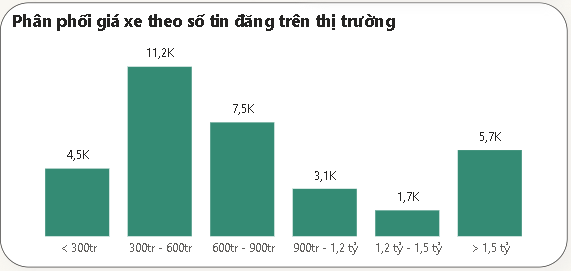
\includegraphics[width=0.8\textwidth]{graphics/Tab02/2.1.PNG}
\caption{Biểu đồ phân phối phân khúc giá xe theo số tin đăng}
\label{fig:tab2_chart_1_1}
\end{figure}

\noindent\textbf{Loại biểu đồ:} Biểu đồ cột dọc.

\begin{itemize}
    \item \textbf{Mục đích và ý nghĩa:} Biểu đồ nhằm xác định phân khúc giá phổ biến nhất, từ đó chứng minh giả thuyết thị trường xe cũ tại Việt Nam chủ yếu được dẫn dắt bởi nhóm khách hàng bình dân và trung lưu.
    
    \item \textbf{Sử dụng dữ liệu:}
    \begin{itemize}
        \item Bảng dữ liệu nguồn: \texttt{fact\_car\_listings}.
        \item Chỉ số: Đếm số lượng \texttt{Mã tin} (Count).
        \item Cột phân nhóm: \texttt{Giá (triệu VND)} (được chia khoảng/bin thành các nhóm: $<$300tr, 300tr - 600tr...).
    \end{itemize}
    
    \item \textbf{Thiết kế và giải thích:} Dạng biểu đồ cột dọc giúp thể hiện trực quan hình dáng phân phối (phân phối lệch phải). Tông màu xanh lục đậm được sử dụng đồng nhất, trong đó cột cao nhất được nhấn mạnh ngầm bằng kích thước áp đảo, điều hướng mắt người xem ngay lập tức vào phân khúc trọng tâm.
    
    \item \textbf{Mã hóa trực quan:}
    \begin{itemize}
        \item Trục ngang (X): Các phân khúc giá tăng dần từ trái sang phải.
        \item Trục dọc (Y): Số lượng tin đăng (K = Nghìn).
        \item Nhãn dữ liệu: Hiển thị trực tiếp con số trên đỉnh mỗi cột (VD: 11,2K) để người đọc không phải gióng sang trục Y.
    \end{itemize}
    
    \item \textbf{Nhận định và phân tích:}
    \begin{itemize}
        \item Thứ bậc và tỷ trọng chính: Phân khúc 300 - 600 triệu đồng chiếm số lượng áp đảo với 11.200 tin đăng, xếp sau là phân khúc 600 - 900 triệu (7.500 tin).
        \item Bối cảnh và lý giải: Đây là tầm giá lý tưởng để mua các dòng xe hạng A, B, C hoặc xe gầm cao đời cũ. Điều này phản ánh thu nhập trung bình và nhu cầu sở hữu ô tô lần đầu của phần lớn các gia đình Việt Nam. 
    \end{itemize}
\end{itemize}

% --- Biểu đồ 1.2 ---
\begin{figure}[H]
\centering
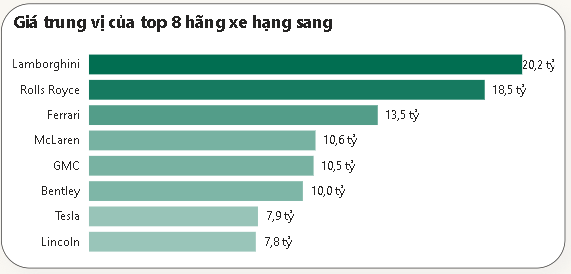
\includegraphics[width=0.8\textwidth]{graphics/Tab02/2.2.PNG}
\caption{Giá trung vị của top 8 hãng xe hạng sang}
\label{fig:tab2_chart_1_2}
\end{figure}

\noindent\textbf{Loại biểu đồ:} Biểu đồ thanh ngang.

\begin{itemize}
    \item \textbf{Mục đích và ý nghĩa:} Mở rộng vào góc khuất cực đoan của thị trường: nhóm xe siêu sang nhằm giúp xác định mức định giá trần mà giới siêu giàu đang chi trả.
    
    \item \textbf{Sử dụng dữ liệu:}
    \begin{itemize}
        \item Bảng dữ liệu nguồn: \texttt{fact\_car\_listings} và \texttt{dim\_brand}.
        \item Chỉ số: Giá trung vị tính từ cột \texttt{Giá (triệu VND)}.
        \item Điều kiện lọc: Chỉ lọc lấy Top 8 hãng xe có giá trị trung vị cao nhất.
    \end{itemize}
    
    \item \textbf{Thiết kế và giải thích:} Biểu đồ thanh ngang giúp dễ dàng đọc tên các hãng xe dài. Ứng dụng kỹ thuật ``Gradient màu'' (nhạt dần từ trên xuống dưới) tạo hiệu ứng thị giác phân cấp mạnh mẽ, tập trung sự chú ý vào hãng xe đắt đỏ nhất.
    
    \item \textbf{Nhận định và phân tích:}
    \begin{itemize}
        \item Thứ bậc và tỷ trọng chính: Lamborghini đứng đầu bảng với mức giá trung vị lên tới 20,2 tỷ đồng, bám sát theo sau là Rolls-Royce với 18,5 tỷ đồng.
        \item Chênh lệch: Có sự ngắt quãng khá rõ giữa Top 3 (trên 13 tỷ) so với phần còn lại của nhóm hạng sang (quanh mốc 10 tỷ).
    \end{itemize}
\end{itemize}

\noindent\textbf{Kết luận và đề xuất hành động cho câu hỏi 1:} 
\begin{itemize}
    \item \textbf{Đúc kết cốt lõi:} Thị trường ô tô Việt Nam phân hóa rất mạnh. Trong khi đại đa số (hơn 50\%) xoay quanh phân khúc bình dân 300 - 900 triệu, thị trường vẫn tồn tại một tầng lớp siêu sang vươn tới mức giá hàng chục tỷ đồng.
    \item \textbf{Đề xuất hành động:} 
    \begin{itemize}
        \item \textbf{Với đại lý bán lẻ:} Nên tập trung tối đa dòng tiền nhập hàng vào phân khúc 300 - 900 triệu vì thanh khoản cao nhất. 
        \item \textbf{Với các nền tảng đăng tin:} Cần có giao diện hoặc khu vực riêng biệt (VIP) để hiển thị nhóm xe siêu sang nhằm thu hút tập khách hàng ngách có tài chính lớn.
    \end{itemize}
\end{itemize}


% ------------------------------------------------------------------------------
% 5.2.4 CÂU HỎI SMART 2
% ------------------------------------------------------------------------------
\subsubsection{Câu hỏi 2}
\label{subsubsec:tab2_q2}
\noindent \textbf{Nội dung câu hỏi: Giá trị của phương tiện khấu hao như thế nào theo tuổi đời (năm sản xuất) và cường độ sử dụng (số kilomet)?}

\begin{figure}[H]
\centering
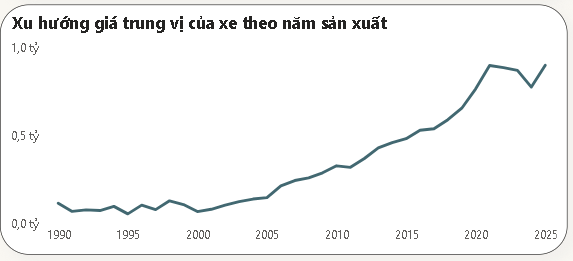
\includegraphics[width=0.8\textwidth]{graphics/Tab02/2.3.PNG}
\caption{Xu hướng biến động giá trung vị của xe theo năm sản xuất (1990 - 2025)}
\label{fig:tab2_chart_2_1}
\end{figure}

\noindent\textbf{Loại biểu đồ:} Biểu đồ đường.

\begin{itemize}
    \item \textbf{Mục đích và ý nghĩa:} Đánh giá độ dốc của sự mất giá phương tiện qua từng năm, giúp trả lời câu hỏi xe giữ giá được bao lâu trước khi chạm đáy khấu hao.
    
    \item \textbf{Sử dụng dữ liệu:}
    \begin{itemize}
        \item Bảng dữ liệu nguồn: \texttt{fact\_car\_listings}.
        \item Chỉ số: Giá trung vị tính từ cột \texttt{Giá (triệu VND)}.
        \item Phân nhóm thời gian (Trục X): \texttt{Năm sản xuất}.
    \end{itemize}
    
    \item \textbf{Thiết kế và giải thích:} Biểu đồ đường là lựa chọn hoàn hảo nhất để quan sát dữ liệu chuỗi thời gian. Đường biểu diễn đậm nét, liên tục, loại bỏ hoàn toàn các đường lưới rối rắm để tối ưu hóa tỷ lệ Data-ink.
    
    \item \textbf{Nhận định và phân tích:}
    \begin{itemize}
        \item Xu hướng: Giá xe rớt dốc cực mạnh ở 5 - 7 năm đầu tiên (từ 2025 lùi về 2018), sau đó đồ thị đi ngang (chạm đáy khấu hao) đối với các xe sản xuất trước năm 2005 (giá chỉ còn dao động dưới 200 triệu).
        \item Bối cảnh: Xe ô tô là tiêu sản. Các công nghệ mới liên tục ra mắt khiến các dòng xe đời cũ nhanh chóng mất đi giá trị ban đầu.
    \end{itemize}
\end{itemize}

% --- Biểu đồ 2.2 ---
\begin{figure}[H]
\centering
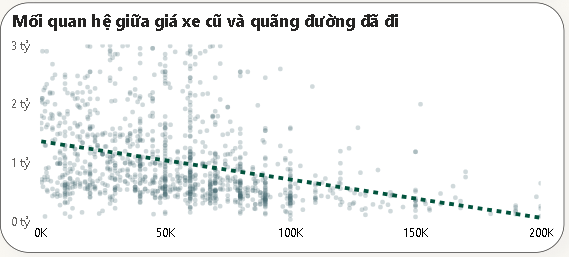
\includegraphics[width=0.8\textwidth]{graphics/Tab02/2.4.PNG}
\caption{Mối quan hệ tương quan giữa giá bán và quãng đường đã di chuyển}
\label{fig:tab2_chart_2_2}
\end{figure}

\noindent\textbf{Loại biểu đồ:} Biểu đồ phân tán kết hợp đường xu hướng.

\begin{itemize}
    \item \textbf{Mục đích và ý nghĩa:} Kiểm chứng mức độ ảnh hưởng của cường độ vận hành (số km thực tế) lên giá bán xe cũ, loại bỏ yếu tố thời gian.
    
    \item \textbf{Sử dụng dữ liệu:}
    \begin{itemize}
        \item Bảng dữ liệu nguồn: \texttt{fact\_car\_listings}.
        \item Trục X: \texttt{Số Km đã đi sạch}.
        \item Trục Y: \texttt{Giá (triệu VND)}.
        \item Điều kiện lọc: Lọc \texttt{Tình trạng} = ``Xe đã dùng'' (chỉ khảo sát xe cũ).
    \end{itemize}
    
    \item \textbf{Thiết kế và giải thích:} Dùng kỹ thuật giảm độ mờ các điểm chấm xuống 30 - 50\% để xử lý tình trạng chồng chéo dữ liệu. Điểm nhấn là đường trendline nét đứt màu đậm cắt ngang đồ thị, chỉ ra rõ rệt hướng đi của dữ liệu.
    
    \item \textbf{Nhận định và phân tích:}
    \begin{itemize}
        \item Xu hướng: Tương quan nghịch biến rõ ràng. Đường xu hướng cắm thẳng xuống từ mốc 0 km đến 200.000 km, xác nhận rằng xe đi càng nhiều, giá trị càng thấp.
        \item Phân tán: Tuy nhiên, các điểm dữ liệu khá vỡ vụn quanh đường xu hướng. Điều này chứng tỏ số Km không phải là yếu tố duy nhất định giá xe (một chiếc xe đi nhiều nhưng hãng sang, bảo dưỡng tốt vẫn có giá cao hơn xe đi ít của hãng giá rẻ).
    \end{itemize}
\end{itemize}

\noindent\textbf{Kết luận và đề xuất hành động cho câu hỏi 2:} 
\begin{itemize}
    \item \textbf{Đúc kết cốt lõi:} Tuổi đời và cường độ khai thác là ``kẻ thù'' lớn nhất bào mòn giá trị ô tô. Đặc biệt, tốc độ mất giá diễn ra tàn khốc nhất trong 5 năm đầu tiên kể từ lúc mua mới.
    \item \textbf{Đề xuất hành động:} 
    \begin{itemize}
        \item \textbf{Với người mua xe cũ:} Nên ưu tiên tìm kiếm những chiếc xe có tuổi đời từ 4 - 6 năm. Đây là thời điểm vàng khi xe đã chịu xong phần khấu hao nặng nề nhất từ chủ cũ nhưng máy móc, công nghệ vẫn còn rất mới.
        \item \textbf{Với người bán (chủ xe):} Nếu muốn tối ưu hóa thu hồi vốn, nên bán xe trước khi chạm mốc 5 năm tuổi hoặc trước khi ODO vượt quá 100.000 km để tránh bị rớt hạng định giá.
    \end{itemize}
\end{itemize}



% ------------------------------------------------------------------------------

% ------------------------------------------------------------------------------
% 5.2.5 TỔNG KẾT VÀ INSIGHT CHIẾN LƯỢC CẤP TAB
% ------------------------------------------------------------------------------
\subsubsection{Tổng kết và định hướng chiến lược cho Tab 2}
\label{subsubsec:tab2_summary}

\noindent\textbf{Tổng hợp các insights chính:}
\begin{itemize}
    \item \textbf{Insight từ câu hỏi 1:} Cấu trúc thị trường phân hóa hình tháp. Đáy tháp cực lớn là phân khúc xe bình dân và trung lưu (dưới 900 triệu đồng) phục vụ nhu cầu đi lại cơ bản. Tuy nhiên, đỉnh tháp lại vươn rất cao với nhóm xe siêu sang (như Lamborghini, Rolls-Royce) chạm mốc trung vị trên 18 tỷ đồng, phục vụ nhu cầu thể hiện đẳng cấp của giới siêu giàu.
    \item \textbf{Insight từ câu hỏi 2:} Xe ô tô là tiêu sản với chu kỳ rớt giá khắc nghiệt. Biểu đồ đường và biểu đồ phân tán cùng chỉ ra rằng: 5 năm đầu tiên và mốc 100.000 km là hai ``ngưỡng cản'' tàn phá giá trị chiếc xe mạnh mẽ nhất, trước khi đồ thị đi ngang và tài sản chạm đáy khấu hao.
\end{itemize}

\noindent\textbf{Trả lời câu hỏi tổng thể:} 
Mức giá hợp lý trên thị trường ô tô Việt Nam xoay quanh mốc trung vị 638 triệu đồng. Mức định giá này không cố định mà bị chi phối mạnh mẽ bởi quy luật khấu hao thời gian và cường độ vận hành. Những chiếc xe lướt (mới sử dụng 1 - 3 năm) chịu mức tổn thất giá trị cao nhất so với giá niêm yết ban đầu, tạo ra khoảng hở chênh lệch lớn mang lại lợi ích cho người mua sau.

\noindent\textbf{Khuyến nghị và hàm ý thực tiễn:}
\begin{itemize}
    \item \textbf{Đối với người mua:} 
    Để tối ưu bài toán kinh tế, tuyệt đối không nên mua xe mới đập hộp nếu ngân sách hạn hẹp. Hãy săn tìm những chiếc xe cũ nằm trong khoảng tối ưu (sản xuất cách đây 4 - 5 năm, ODO dưới 60.000 km) để hưởng trọn phần khấu hao mà chủ cũ đã gánh chịu, trong khi chất lượng xe vẫn còn rất tốt.
    \item \textbf{Đối với người bán:} 
    Nếu có ý định lên đời xe, hãy rao bán phương tiện trước khi nó vượt qua các mốc rớt giá tâm lý nguy hiểm (xe quá 5 năm tuổi hoặc ODO chớm mốc 100.000 km) để có thể thỏa thuận được mức giá hời nhất.
\end{itemize}





\subsection{Mục tiêu 3: Cuộc chiến xe xăng và điện}
\label{subsec:tab3}

% ------------------------------------------------------------------------------
% 5.3.1 BỐI CẢNH VÀ MÔ HÌNH DỮ LIỆU CỦA TAB
% ------------------------------------------------------------------------------
\subsubsection{Bối cảnh phân tích và mô hình dữ liệu}
\label{subsubsec:tab3_schema}

\noindent\textbf{Bối cảnh và mục tiêu phân tích:}
Tab 3 giải quyết một trong những chủ đề nóng nhất của ngành công nghiệp ô tô hiện nay là cuộc cạnh tranh giữa xe sử dụng động cơ đốt trong truyền thống và xe năng lượng mới. Nội dung tập trung làm rõ liệu xe điện chỉ là một trào lưu nhất thời hay thực sự đang định hình lại cấu trúc thị trường. Qua đó, phân tích này đóng góp vào câu hỏi cốt lõi của đồ án bằng cách làm sáng tỏ chiến lược định giá và mức độ tiếp nhận của người tiêu dùng đối với xe năng lượng xanh.

\noindent\textbf{Bảng tổng hợp danh sách trường dữ liệu khai thác:}
\begin{table}[H]
\centering
\small
\begin{tabularx}{\textwidth}{L{3cm} L{3.5cm} L{4.5cm} Y}
\hline
\textbf{Tên cột} & \textbf{Bảng nguồn} & \textbf{Ý nghĩa dữ liệu} & \textbf{Phục vụ phân tích} \\ \hline
Mã tin & fact\_car\_listings & Mã định danh tin đăng bán xe & Biến đo lường (Đếm số lượng) \\ \hline
Nhiên liệu & fact\_car\_listings & Loại năng lượng phương tiện sử dụng (xăng, điện, dầu, hybrid) & Phân loại chính \\ \hline
Năm sản xuất & fact\_car\_listings & Tuổi đời của xe & Phân loại / Trục thời gian \\ \hline
Giá (triệu VND) & fact\_car\_listings & Giá bán của phương tiện & Biến đo lường (Trung vị) \\ \hline
Kiểu dáng & dim\_body\_type & Thiết kế thân xe (SUV, Crossover, Hatchback) & Phân loại (So sánh ngang hàng) \\ \hline
Tình trạng & fact\_car\_listings & Tình trạng sử dụng (Mới, Đã dùng) & Phân loại \\ \hline
Tên hãng & dim\_brand & Thương hiệu sản xuất & Bộ lọc (Đo lường thị phần VinFast) \\ \hline
\end{tabularx}
\caption{Danh sách các trường dữ liệu khai thác trong Tab 3}
\label{tab:schema_tab3}
\end{table}


% ------------------------------------------------------------------------------
% 5.3.2 KHỐI CHỈ SỐ KPI TỔNG QUAN
% ------------------------------------------------------------------------------
\subsubsection{Khối chỉ số KPI tổng quan}
\label{subsubsec:tab3_kpi}

\begin{table}[H]
\centering
\small
\begin{tabularx}{\textwidth}{L{2.5cm} L{2cm} L{4.5cm} Y}
\hline
\textbf{Thẻ KPI} & \textbf{Giá trị} & \textbf{Công thức hoặc Logic} & \textbf{Ý nghĩa định hướng} \\ \hline
Quy mô xe điện & 768 & Đếm tổng số tin đăng lọc theo nhiên liệu là điện & Xác nhận tập dữ liệu mẫu đủ lớn để đưa ra các phân tích thống kê có ý nghĩa, tránh thiên lệch do thiếu dữ liệu. \\ \hline
Thị phần năm 2025 & 19.79\% & Tỷ lệ xe điện trên tổng số xe sản xuất năm 2025 & Cho thấy tốc độ chiếm lĩnh thị trường ở mốc thời gian gần nhất, làm cơ sở để đánh giá xu hướng tương lai. \\ \hline
VinFast dẫn đầu & 89\% & Tỷ lệ xe thuộc hãng VinFast trong tổng số xe điện & Khẳng định vai trò dẫn dắt thị trường và mức độ độc quyền của thương hiệu nội địa trong phân khúc này. \\ \hline
\end{tabularx}
\caption{Tổng hợp các chỉ số KPI điều hướng hàng đầu trên Dashboard Tab 3}
\label{tab:kpi_tab3}
\end{table}

% ------------------------------------------------------------------------------
% 5.3.3 CÂU HỎI SMART 1
% ------------------------------------------------------------------------------
\subsubsection{Câu hỏi 1:}
\noindent \textbf{Nội dung câu hỏi: Xe điện chỉ chiếm 2.3\% toàn bộ dữ liệu - vậy tại sao gọi đây là một “cuộc bứt phá”, và điều gì đang âm thầm xảy ra song song mà ít người để ý?}

\begin{figure}[H]
\centering
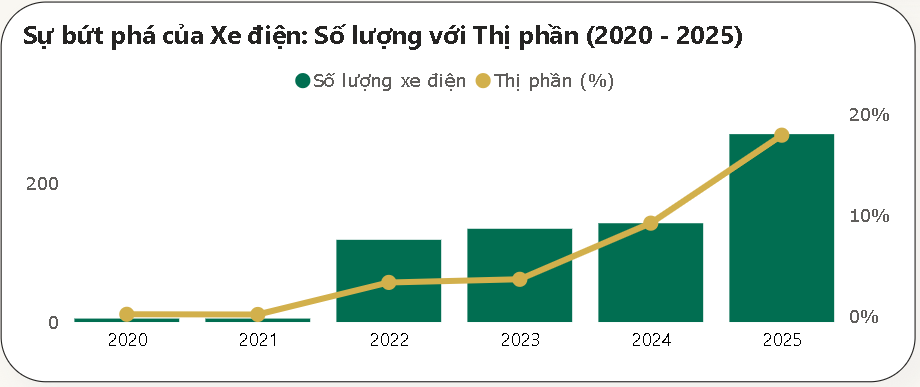
\includegraphics[width=0.8\textwidth]{graphics/Tab03/3.1.PNG}
\caption{Số lượng và thị phần xe điện từ năm 2020 đến 2025}
\label{fig:tab3_chart_5_1}
\end{figure}

\noindent\textbf{Loại biểu đồ:} Biểu đồ kết hợp cột dọc và đường.

\begin{itemize}
    \item \textbf{Mục đích và ý nghĩa:} Biểu đồ giải thích nghịch lý giữa con số tổng lũy kế khiêm tốn (2.3\%) và nhận định về sự bùng nổ của xe điện.
    
    \item \textbf{Sử dụng dữ liệu:}
    \begin{itemize}
        \item Bảng dữ liệu nguồn: \texttt{fact\_car\_listings}.
        \item Chỉ số: Số lượng tin đăng (cột) và tỷ lệ phần trăm (đường).
        \item Điều kiện lọc: Nhiên liệu là điện, năm sản xuất từ 2020 đến 2025.
    \end{itemize}
    
    \item \textbf{Thiết kế và giải thích:} Việc kết hợp cột và đường giúp quan sát đồng thời cả quy mô tuyệt đối lẫn tỷ trọng tương đối. Tông màu xanh lá được sử dụng xuyên suốt để đại diện cho nhóm năng lượng sạch.
    
    \item \textbf{Mã hóa trực quan:}
    \begin{itemize}
        \item Trục ngang: Năm sản xuất tăng dần.
        \item Trục dọc trái: Số lượng xe điện thực tế.
        \item Trục dọc phải: Phần trăm thị phần so với các loại nhiên liệu khác trong cùng năm.
    \end{itemize}
    
    \item \textbf{Nhận định và phân tích:}
    \begin{itemize}
        \item Thứ bậc và xu hướng: Giai đoạn 2020 đến 2021, xe điện gần như vô hình trên bản đồ. Tuy nhiên, từ năm 2022 trở đi, đồ thị đi lên theo chiều dốc đứng. Đến năm 2025, tỷ trọng xe điện đã chạm ngưỡng gần 20\%. 
        \item Bối cảnh và lý giải: Sự bứt phá không nằm ở con số tổng cộng từ quá khứ, mà nằm ở tốc độ tăng trưởng hiện tại. Sự xuất hiện của các dải sản phẩm mới từ thương hiệu nội địa chính là chất xúc tác cho bước nhảy vọt này.
    \end{itemize}
\end{itemize}

\begin{figure}[H]
\centering
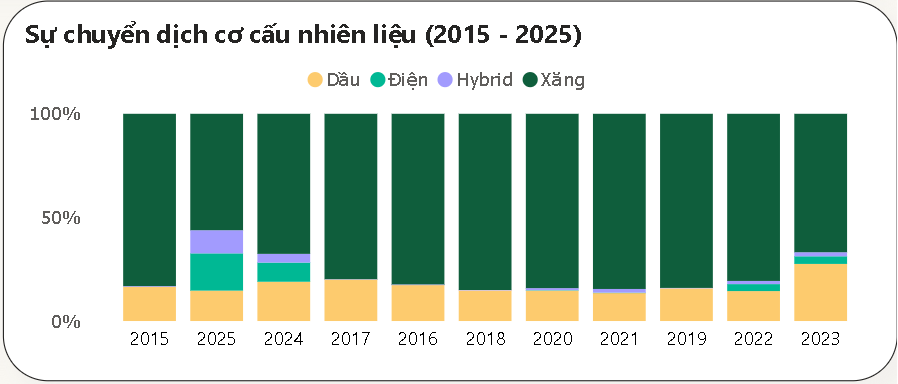
\includegraphics[width=0.8\textwidth]{graphics/Tab03/3.2.PNG}
\caption{Sự chuyển dịch cơ cấu nhiên liệu của thị trường ô tô từ 2015 đến 2025}
\label{fig:tab3_chart_5_2}
\end{figure}

\noindent\textbf{Loại biểu đồ:} Biểu đồ cột chồng 100\%.

\begin{itemize}
    \item \textbf{Mục đích và ý nghĩa:} Trả lời vế sau của câu hỏi bằng cách rõ những thay đổi ngầm trong cơ cấu toàn ngành khi xe điện xuất hiện.
    
    \item \textbf{Sử dụng dữ liệu:}
    \begin{itemize}
        \item Bảng dữ liệu nguồn: \texttt{fact\_car\_listings}.
        \item Chỉ số: Tỷ lệ phần trăm tin đăng.
        \item Phân nhóm: Nhiên liệu (Xăng, Dầu, Hybrid, Điện).
    \end{itemize}
    
    \item \textbf{Thiết kế và giải thích:} Dạng biểu đồ cột chồng 100\% là phương án tối ưu để thấy rõ sự cạnh tranh của thị phần, khi một nhóm tăng lên bắt buộc nhóm khác phải thu hẹp lại.
    
    \item \textbf{Nhận định và phân tích:}
    \begin{itemize}
        \item Sự lấn át: Nhóm xe xăng (màu xanh lục đậm) đang mất dần thế độc tôn từ mốc hơn 80\% ở các năm trước xuống còn tỷ trọng nhỏ hơn hẳn vào năm 2025. 
        \item Diễn biến song song: Đồng hành cùng xe điện, các dòng xe hybrid cũng bắt đầu chiếm một dải mỏng nhưng rõ rệt ở các năm gần đây, minh chứng cho xu hướng người tiêu dùng muốn trải nghiệm điện khí hóa nhưng vẫn cần sự an toàn của động cơ đốt trong.
    \end{itemize}
\end{itemize}

\noindent\textbf{Kết luận và đề xuất hành động cho câu hỏi 1:} 
\begin{itemize}
    \item \textbf{Đúc kết cốt lõi:} Nhìn vào tổng thể toàn bộ lịch sử thị trường thì xe điện vẫn rất bé nhỏ. Tuy nhiên, nếu chỉ tính các xe ra mắt trong ba năm trở lại đây, nhóm xe này đang dần chiếm đi thị phần của xe xăng với tốc độ cực nhanh, đi kèm sự xuất hiện của dòng xe hybrid.
    \item \textbf{Đề xuất hành động:} Các hệ thống garage sửa chữa và dịch vụ bảo dưỡng cần nhanh chóng bổ sung nhân sự và thiết bị chẩn đoán chuyên dụng cho xe điện và hybrid. Nhóm kinh doanh phụ tùng truyền thống sẽ bắt đầu thấy doanh số chững lại trong 3 đến 5 năm tới.
\end{itemize}

% ------------------------------------------------------------------------------
% 5.3.4 CÂU HỎI SMART 2
% ------------------------------------------------------------------------------
\subsubsection{Câu hỏi 2:}
\label{subsubsec:tab3_q6}
\noindent \textbf{Nội dung câu hỏi: Quan niệm phổ biến cho rằng xe điện đắt hơn và được giữ dùng lâu dài, dữ liệu thực tế có xác nhận điều này không?}

\begin{figure}[H]
\centering
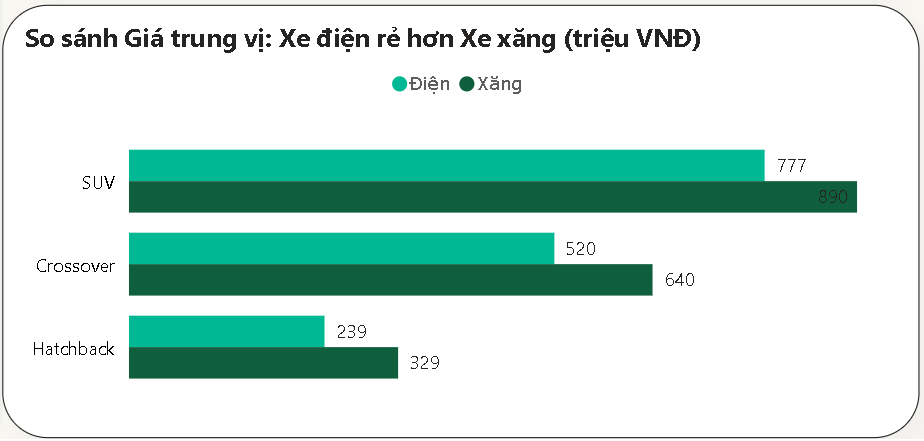
\includegraphics[width=0.8\textwidth]{graphics/Tab03/3.3.PNG}
\caption{So sánh giá trung vị giữa xe điện và xe xăng}
\label{fig:tab3_chart_6_1}
\end{figure}

\noindent\textbf{Loại biểu đồ:} Biểu đồ thanh ngang ghép nhóm.

\begin{itemize}
    \item \textbf{Mục đích và ý nghĩa:} Kiểm chứng định kiến của thị trường cho rằng chi phí sở hữu xe điện luôn cao hơn xe xăng do giá thành pin.
    
    \item \textbf{Sử dụng dữ liệu:}
    \begin{itemize}
        \item Bảng dữ liệu nguồn: \texttt{fact\_car\_listings} và \texttt{dim\_body\_type}.
        \item Chỉ số: Giá trung vị.
        \item Phân nhóm: Nhiên liệu (chỉ lấy Xăng và Điện) và Kiểu dáng (SUV, Crossover, Hatchback).
    \end{itemize}
    
    \item \textbf{Thiết kế và giải thích:} Việc đặt hai thanh ngang cạnh nhau cho từng nhóm kiểu dáng tạo ra sự so sánh trực quan, không qua trung gian.
    
    \item \textbf{Nhận định và phân tích:}
    \begin{itemize}
        \item Chênh lệch giá: Ở mọi phân khúc được khảo sát, giá trung vị của xe điện luôn thấp hơn xe xăng. Điển hình ở phân khúc Hatchback, xe điện có giá trung bình 239 triệu, rẻ hơn rõ rệt so với mức 329 triệu của xe xăng.
        \item Lý giải: Kết quả này phản ánh chính sách định giá mang tính thâm nhập thị trường của nhà sản xuất, kết hợp với các hình thức bán xe không kèm pin giúp giảm chi phí mua ban đầu xuống mức rất dễ tiếp cận.
    \end{itemize}
\end{itemize}

\begin{figure}[H]
\centering
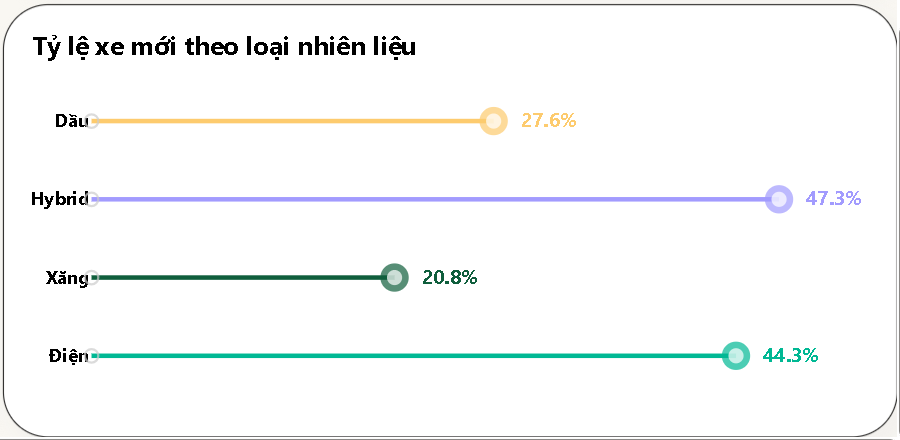
\includegraphics[width=0.8\textwidth]{graphics/Tab03/3.4.PNG}
\caption{Tỷ lệ xe mới được bán theo loại nhiên liệu}
\label{fig:tab3_chart_6_2}
\end{figure}

\noindent\textbf{Loại biểu đồ:} Biểu đồ kẹo mút.

\begin{itemize}
    \item \textbf{Mục đích và ý nghĩa:} Kiểm tra xem người dùng có thực sự giữ xe điện lại để dùng lâu dài như các loại tài sản lớn thông thường hay không.
    
    \item \textbf{Sử dụng dữ liệu:}
    \begin{itemize}
        \item Bảng dữ liệu nguồn: \texttt{fact\_car\_listings}.
        \item Chỉ số: Tỷ lệ phần trăm các tin đăng có Tình trạng là \texttt{mới}.
        \item Phân nhóm: Nhiên liệu.
    \end{itemize}
    
    \item \textbf{Thiết kế và giải thích:} Lược bỏ các cột dày đặc, chỉ giữ lại một thanh mỏng và một điểm tròn có nhãn số liệu, giúp hình ảnh trông thanh thoát hơn và đi thẳng vào kết quả cuối cùng.
    
    \item \textbf{Nhận định và phân tích:}
    \begin{itemize}
        \item Khoảng cách chênh lệch: Lên tới 44.3\% lượng tin đăng xe điện là xe mới chưa lăn bánh, con số này cao gấp đôi so với xe xăng (chỉ 20.8\%). Nhóm hybrid cũng ghi nhận tỷ lệ bán mới rất cao ở mức 47.3\%.
        \item Lý giải: Điều này cho thấy xe năng lượng mới đang có vòng đời đẩy hàng ra thị trường rất nhanh. Lượng lớn tin đăng đến từ các đại lý xả kho hoặc người dùng mua đi bán lại các xe vừa xuất xưởng để chênh lệch giá, phản bác lại quan niệm mua xe điện để gắn bó lâu dài.
    \end{itemize}
\end{itemize}

\noindent\textbf{Kết luận và đề xuất hành động cho câu hỏi 2:} 
\begin{itemize}
    \item \textbf{Đúc kết cốt lõi:} Dữ liệu đã phủ nhận hai định kiến lớn nhất. Xe điện không hề đắt đỏ hơn xe xăng nếu xét cùng phân khúc, và chúng đang tạo ra một xu hướng giao dịch xe mới cực kì sôi động chứ không cố định trong gara của người dùng.
    \item \textbf{Đề xuất hành động:} Người mua có ngân sách hẹp nên cân nhắc chọn xe điện ở phân khúc Hatchback và Crossover để tối ưu chi phí đầu tư. Các nền tảng giao dịch cần tối ưu bộ lọc tìm kiếm xe lướt, xe mới cho nhóm năng lượng này vì nguồn cung đang rất dồi dào.
\end{itemize}

% ------------------------------------------------------------------------------
% 5.3.5 TỔNG KẾT VÀ INSIGHT CHIẾN LƯỢC CẤP TAB
% ------------------------------------------------------------------------------
\subsubsection{Tổng kết và định hướng chiến lược cho Tab 3}
\label{subsubsec:tab3_summary}

\noindent\textbf{Tổng hợp các insights chính:}
\begin{itemize}
    \item \textbf{Insight từ câu hỏi 1:} Xe điện đang tạo ra cú sốc về tốc độ tăng trưởng ở giai đoạn gần đây, âm thầm bóp nghẹt thị phần của xe xăng và kéo theo sự xuất hiện bước đệm của dòng xe lai.
    \item \textbf{Insight từ câu hỏi 2:} Yếu tố cốt lõi giúp xe điện cạnh tranh thành công là chiến lược giá thấp hơn mặt bằng chung, đi kèm với nguồn cung xe mới dồi dào tạo tính thanh khoản cao.
\end{itemize}

\noindent\textbf{Trả lời câu hỏi tổng thể:} 
Cuộc chiến giữa xe xăng và xe điện không còn ở giai đoạn lý thuyết mà đã hiển hiện trên số liệu giao dịch. Xe điện đang sử dụng chiến lược lấy giá cả làm vũ khí mũi nhọn để thay đổi nhận thức người dùng và định hình lại cấu trúc nguồn cung trong tương lai gần.

\noindent\textbf{Khuyến nghị và hàm ý thực tiễn:}
\begin{itemize}
    \item \textbf{Đối với doanh nghiệp và nhà quản lý:} Các đại lý ô tô truyền thống cần đa dạng hóa danh mục nhập hàng, giảm tỷ lệ phụ thuộc vào xe xăng đời mới để tránh tình trạng tồn kho khi làn sóng xe xanh lan rộng. Cần nghiên cứu phát triển thêm mảng dịch vụ thu mua và thẩm định riêng cho pin xe điện.
    \item \textbf{Đối với người mua:} Khách hàng có thể tận dụng lợi thế về giá để trải nghiệm xe điện ở phân khúc phổ thông. Tuy nhiên, do nguồn cung xe mới rất nhiều, người mua cần tham khảo giá kĩ lưỡng để tránh mua hớ ở các đại lý bán lẻ.
\end{itemize}


\subsection{Mục tiêu 4: Chân dung người mua}
\label{subsec:tab[X]}

% ------------------------------------------------------------------------------
% 5.X.1 BỐI CẢNH VÀ MÔ HÌNH DỮ LIỆU CỦA TAB
% ------------------------------------------------------------------------------
\subsubsection{Bối cảnh phân tích và mô hình dữ liệu}
\label{subsubsec:tab4_schema}

\noindent\textbf{Bối cảnh và mục tiêu phân tích:}
Tab 4: ``Chân dung người mua'' tập trung khắc họa thị hiếu và hành vi lựa chọn cấu hình của người tiêu dùng trên thị trường xe ô tô Việt Nam, bao gồm màu sắc ngoại thất, loại hộp số và số chỗ ngồi. Bên cạnh đó, tab còn đối chiếu với hành vi rao bán lại xe cũ thông qua quãng đường đã đi tại thời điểm đăng tin. Qua đó, tab đóng góp vào câu hỏi cốt lõi: ``người mua xe Việt đang ưu tiên cấu hình nào, và thói quen sử dụng xe đã thay đổi ra sao theo thời gian?''.

\begin{table}[H]
\centering
\small
\begin{tabular}{p{3cm} p{3.5cm} p{4cm} p{3.5cm}}
\textbf{Tên cột} & \textbf{Bảng nguồn} & \textbf{Ý nghĩa dữ liệu} & \textbf{Phục vụ phân tích} \\ \hline
Mã tin & fact\_car\_listings & Mã định danh duy nhất của mỗi tin đăng bán xe & Biến đo lường (đếm số lượng) \\
Màu ngoại thất & fact\_car\_listings & Màu sơn bên ngoài xe do người bán khai báo & Phân loại / So sánh tỷ trọng \\
Loại hộp số & fact\_car\_listings & Hình thức truyền động của xe, số tự động hoặc số sàn & Phân loại / Xu hướng theo năm \\
Số chỗ ngồi & fact\_car\_listings & Số lượng ghế ngồi theo thiết kế của xe & Phân loại / Phân bổ tỷ trọng \\
Năm sản xuất & fact\_car\_listings & Năm xe được sản xuất, dùng làm trục thời gian cho xu hướng chuyển dịch hộp số & Trục tọa độ (X) \\
Số Km đã đi sạch & fact\_car\_listings & Quãng đường thực tế xe đã lăn bánh tại thời điểm rao bán lại & Biến đo lường (trung vị) \\
Năm đăng tin & fact\_car\_listings & Thời điểm tin rao bán được đăng lên hệ thống & Trục tọa độ (X) \\
\end{tabular}
\caption{Các trường dữ liệu khai thác}
\label{tab:schema_tab4}
\end{table}

% ------------------------------------------------------------------------------
% khối chỉ số kpi tổng quan
% ------------------------------------------------------------------------------
\subsubsection{Khối chỉ số KPI tổng quan}
\label{subsubsec:tab4_kpi}

\begin{table}[H]
\centering
\small
\begin{tabular}{p{2cm} p{2cm} p{4.5cm} p{5cm}}
\textbf{Thẻ KPI} & \textbf{Giá trị ghi nhận} & \textbf{Công thức hoặc logic} & \textbf{Ý nghĩa định hướng} \\ \hline
Chọn màu trắng & 33,62\% & Tỷ lệ số tin đăng có màu ngoại thất trắng trên tổng số tin đăng & Xác định gu thẩm mỹ chủ đạo của người mua xe Việt, làm cơ sở tham khảo cho đại lý khi nhập hàng theo màu sắc. \\
Chọn số tự động & 82,05\% & Tỷ lệ số tin đăng sử dụng hộp số tự động trên tổng số tin đăng & Cho thấy mức độ phổ biến áp đảo của hộp số tự động, phản ánh sự dịch chuyển thói quen lái xe trong giai đoạn gần đây. \\
Chọn xe 5 chỗ & 68,82\% & Tỷ lệ số tin đăng có cấu hình 5 chỗ ngồi trên tổng số tin đăng & Khẳng định nhu cầu chủ yếu tập trung vào xe cá nhân hoặc gia đình nhỏ, thay vì xe nhiều chỗ phục vụ gia đình lớn hoặc kinh doanh. \\
\end{tabular}
\caption{Các chỉ số KPI điều hướng trên dashboard}
\label{tab:kpi_tab4}
\end{table}
% ------------------------------------------------------------------------------
% 5.X.3 CÂU HỎI SMART 1 (CẤU TRÚC LẶP LẠI CHO Q1, Q2, Q3)
% ------------------------------------------------------------------------------
\subsubsection{Câu hỏi 1}
\label{subsubsec:tab4_q1}

\noindent \textbf{Nội dung câu hỏi: Thị trường ô tô ngày càng đa dạng màu sắc và kiểu dáng, nhưng người mua xe Việt lại ngày càng giống nhau trong lựa chọn, đâu là lý do đằng sau sự đồng nhất bất thường này?}

\begin{figure}[H]
\centering
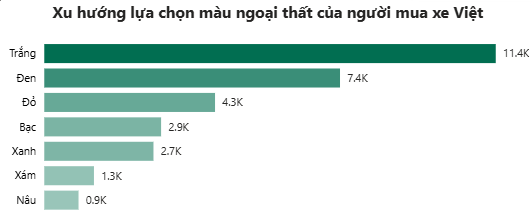
\includegraphics[width=0.8\textwidth]{graphics/Tab04/4.1.PNG}
\caption{Xu hướng lựa chọn màu ngoại thất của người mua xe Việt}
\label{fig:tab4_chart_1_1}
\end{figure}

\noindent\textbf{Loại biểu đồ:} Biểu đồ thanh ngang.

\begin{itemize}
    \item \textbf{Mục đích và ý nghĩa:} Biểu đồ nhằm xác định gu thẩm mỹ chủ đạo của người mua xe Việt, từ đó cung cấp cơ sở tham khảo cho đại lý khi cân đối tỷ trọng màu sắc nhập hàng.
    
    \item \textbf{Sử dụng dữ liệu:}
    \begin{itemize}
        \item Bảng dữ liệu nguồn: \texttt{fact\_car\_listings}.
        \item Chỉ số: Đếm số lượng \texttt{Mã tin} (Count).
        \item Cột phân nhóm: \texttt{Màu ngoại thất}, sắp xếp giảm dần theo số lượng tin đăng.
    \end{itemize}
    
    \item \textbf{Thiết kế và giải thích:} Dạng biểu đồ thanh ngang giúp liệt kê rõ tên các nhóm màu mà không bị chồng chéo nhãn. Tông màu xanh lục được giữ đồng nhất trên toàn bộ các thanh, tránh dùng chính màu sắc thực tế của xe để làm màu biểu đồ vì có thể gây nhiễu thị giác và khó đọc với một số màu nhạt.
    
    \item \textbf{Mã hóa trực quan:}
    \begin{itemize}
        \item Trục dọc (Y): Danh sách các nhóm màu ngoại thất, sắp xếp từ phổ biến nhất đến ít phổ biến nhất.
        \item Trục ngang (X): Số lượng tin đăng tương ứng với mỗi màu.
        \item Nhãn dữ liệu: Hiển thị trực tiếp con số cuối mỗi thanh (VD: 11,4K) để người đọc không phải gióng sang trục X.
    \end{itemize}
    
    \item \textbf{Nhận định và phân tích:}
    \begin{itemize}
        \item Thứ bậc và tỷ trọng chính: Màu trắng dẫn đầu tuyệt đối với 11.400 tin đăng, bỏ xa màu đen ở vị trí thứ hai với 7.400 tin. Nhóm màu trung tính (trắng, đen, bạc, xám) chiếm phần lớn thị phần, trong khi các màu cá tính như đỏ hay xanh chỉ chiếm tỷ trọng nhỏ.
        \item Bối cảnh và lý giải: Xu hướng nghiêng mạnh về màu trung tính phản ánh tâm lý ưu tiên giá trị bán lại và độ trung tính thẩm mỹ khi mua xe tại Việt Nam, thay vì thể hiện cá tính qua màu sắc nổi bật.
        \item Hạn chế: Biểu đồ hiện chỉ thể hiện tỷ trọng tổng gộp toàn bộ giai đoạn, chưa tách theo từng năm nên chưa thể khẳng định mức độ ổn định của thị hiếu màu sắc qua thời gian như câu hỏi đặt ra. Cần bổ sung một biểu đồ xu hướng theo năm sản xuất nếu muốn trả lời trọn vẹn phần này.
    \end{itemize}
\end{itemize}



% ------------------------------------------------------------------------------
% 5.X.4 CÂU HỎI SMART 2
% ------------------------------------------------------------------------------
\begin{figure}[H]
\centering
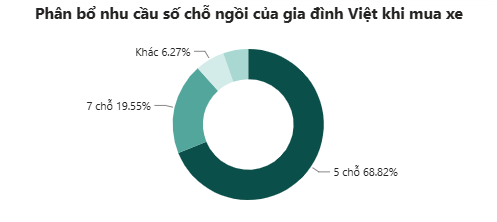
\includegraphics[width=0.8\textwidth]{graphics/Tab04/4.3.PNG}
\caption{Phân bổ nhu cầu số chỗ ngồi của gia đình Việt khi mua xe}
\label{fig:tab4_chart_3_1}
\end{figure}

\noindent\textbf{Loại biểu đồ:} Biểu đồ tròn dạng vành khuyên (donut chart).

\begin{itemize}
    \item \textbf{Mục đích và ý nghĩa:} Biểu đồ nhằm xác định cấu hình số chỗ ngồi chiếm ưu thế trên thị trường, từ đó suy luận nhu cầu sử dụng chủ đạo là xe cá nhân, gia đình nhỏ hay gia đình nhiều thành viên.

    \item \textbf{Sử dụng dữ liệu:}
    \begin{itemize}
        \item Bảng dữ liệu nguồn: \texttt{fact\_car\_listings}.
        \item Chỉ số: Đếm số lượng \texttt{Mã tin}, quy đổi thành tỷ lệ phần trăm trên tổng số tin đăng.
        \item Cột phân nhóm: \texttt{Số chỗ ngồi}, được gom thành các nhóm chính là 5 chỗ, 7 chỗ và khác.
    \end{itemize}

    \item \textbf{Thiết kế và giải thích:} Dạng biểu đồ vành khuyên phù hợp để thể hiện tỷ trọng cấu thành của một tổng thể khi số lượng nhóm phân loại ít. Khoảng trống ở tâm biểu đồ tạo cảm giác nhẹ nhàng hơn so với biểu đồ tròn truyền thống và có thể tận dụng để đặt tổng số tin đăng nếu cần.

    \item \textbf{Mã hóa trực quan:}
    \begin{itemize}
        \item Góc cung: Tỷ lệ phần trăm tương ứng với mỗi nhóm số chỗ ngồi.
        \item Màu sắc: Mỗi nhóm số chỗ ngồi được gán một tông màu xanh riêng biệt, đậm nhạt giảm dần theo tỷ trọng.
        \item Nhãn dữ liệu: Hiển thị trực tiếp tên nhóm và tỷ lệ phần trăm cạnh mỗi phần cung (VD: 5 chỗ 68,82\%).
    \end{itemize}

    \item \textbf{Nhận định và phân tích:}
    \begin{itemize}
        \item Thứ bậc và tỷ trọng chính: Xe 5 chỗ chiếm tỷ trọng áp đảo với 68,82\%, gấp hơn ba lần so với xe 7 chỗ chỉ chiếm 19,55\%, phần còn lại 6,27\% thuộc về các cấu hình khác.
        \item Bối cảnh và lý giải: Tỷ trọng nghiêng mạnh về xe 5 chỗ phản ánh nhu cầu chủ đạo của thị trường vẫn là xe phục vụ cá nhân hoặc gia đình nhỏ, trong khi phân khúc xe 7 chỗ phục vụ gia đình đông thành viên hoặc kinh doanh dịch vụ chỉ chiếm một phần nhỏ.
    \end{itemize}
\end{itemize}

\noindent\textbf{Kết luận và đề xuất hành động cho câu hỏi 1:} 
\begin{itemize}
    \item \textbf{Đúc kết cốt lõi:} Người mua xe Việt Nam đang thể hiện sự đồng nhất bất thường trong 2 lựa chọn tưởng chừng mang tính cá nhân, màu ngoại thất và số chỗ ngồi. Về màu sắc, nhóm màu trung tính (Trắng, Đen) chiếm ưu thế tuyệt đối so với các lựa chọn còn lại. Về cấu hình, nhu cầu tập trung chủ yếu vào xe 5 chỗ phục vụ cá nhân và gia đình nhỏ, trong khi phân khúc nhiều chỗ chỉ giữ vai trò thứ yếu. Cả hai xu hướng cùng phản ánh một tâm lý tiêu dùng thực dụng: người mua đang cân nhắc khả năng thanh khoản khi bán lại và chi phí sử dụng, thay vì thuần túy theo gu thẩm mỹ hay quy mô gia đình lớn.
    \item \textbf{Đề xuất hành động:} 
    \begin{itemize}
        \item \textbf{Với đại lý bán lẻ:} Nên ưu tiên tỷ trọng nhập xe màu trắng và đen ở mức cao nhất vì đây là nhóm có khả năng thanh khoản nhanh nhất, đồng thời duy trì tỷ trọng xe 5 chỗ ở mức cao nhất, chỉ giữ một lượng vừa phải xe 7 chỗ cho nhóm khách hàng gia đình lớn hoặc chạy dịch vụ.
        \item \textbf{Với nhóm phân tích:} Cần bổ sung biểu đồ tách theo năm sản xuất để xác nhận liệu thị hiếu màu trắng có đang tiếp tục tăng hay đã bắt đầu bão hòa, đồng thời có thể tách thêm nhóm 7 chỗ theo dòng xe (SUV, MPV, Van) để hiểu rõ hơn phân khúc này đang phục vụ nhu cầu gia đình hay kinh doanh.
    \end{itemize}
\end{itemize}


\subsubsection{Câu hỏi 2}
\label{subsubsec:tab4_q2}

\noindent \textbf{Nội dung câu hỏi: Điều gì xảy ra khi một thế hệ người mua xe đồng loạt chuyển sang số tự động và cũng đồng loạt bán xe sớm hơn — liệu đây là 2 xu hướng độc lập, hay cùng phản ánh một cách tiêu dùng xe đang thay đổi tận gốc?}

\begin{figure}[H]
\centering
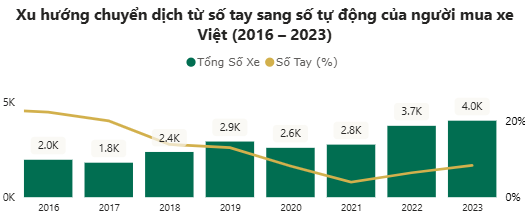
\includegraphics[width=0.8\textwidth]{graphics/Tab04/4.2.PNG}
\caption{Xu hướng chuyển dịch từ số tay sang số tự động của người mua xe Việt (2016 - 2023)}
\label{fig:tab4_chart_2_1}
\end{figure}

\noindent\textbf{Loại biểu đồ:} Biểu đồ kết hợp cột và đường (combo chart).

\begin{itemize}
    \item \textbf{Mục đích và ý nghĩa:} Biểu đồ nhằm lượng hóa tốc độ dịch chuyển công nghệ truyền động, đồng thời đối chiếu quy mô thị trường qua từng năm để tránh nhận định sai lệch khi tỷ lệ phần trăm biến động trên nền số lượng nhỏ.
    
    \item \textbf{Sử dụng dữ liệu:}
    \begin{itemize}
        \item Bảng dữ liệu nguồn: \texttt{fact\_car\_listings}.
        \item Chỉ số cột: Tổng số xe, đếm số lượng \texttt{Mã tin} theo từng năm sản xuất.
        \item Chỉ số đường: Tỷ lệ phần trăm xe số tay trên tổng số xe của năm tương ứng.
        \item Cột phân nhóm: \texttt{Năm sản xuất} (2016 đến 2023), \texttt{Loại hộp số}.
    \end{itemize}
    
    \item \textbf{Thiết kế và giải thích:} Kết hợp cột và đường trên cùng một biểu đồ giúp thể hiện đồng thời hai chiều thông tin, quy mô tuyệt đối (cột) và tỷ trọng tương đối (đường), mà không cần hai biểu đồ tách rời. Trục phụ bên phải dành riêng cho tỷ lệ phần trăm giúp đường xu hướng không bị nén sát đáy biểu đồ.
    
    \item \textbf{Mã hóa trực quan:}
    \begin{itemize}
        \item Trục ngang (X): Năm sản xuất, từ 2016 đến 2023.
        \item Trục dọc trái (Y1): Tổng số xe (đơn vị nghìn).
        \item Trục dọc phải (Y2): Tỷ lệ phần trăm xe số tay.
        \item Nhãn dữ liệu: Hiển thị trực tiếp giá trị trên mỗi cột (VD: 4,0K năm 2023) để người đọc không phải gióng sang trục Y1.
    \end{itemize}
    
    \item \textbf{Nhận định và phân tích:}
    \begin{itemize}
        \item Thứ bậc và tỷ trọng chính: Tổng số xe tăng dần đều qua các năm, từ 2,0K năm 2016 lên 4,0K năm 2023, cho thấy quy mô nguồn cung xe đời mới trên hệ thống ngày càng lớn.
        \item Xu hướng đường tỷ lệ số tay: Đường tỷ lệ xe số tay có xu hướng giảm dần theo thời gian, phản ánh việc hộp số tự động ngày càng chiếm ưu thế trong các đời xe sản xuất gần đây.
        \item Hạn chế: Biểu đồ hiện chưa gắn nhãn phần trăm cụ thể tại từng điểm trên đường xu hướng, khiến việc đọc chính xác mức độ dịch chuyển giữa các năm gặp khó khăn, và cũng chưa tách theo hãng xe để so sánh tốc độ chuyển đổi giữa các thương hiệu.
    \end{itemize}
\end{itemize}



\begin{figure}[H]
\centering
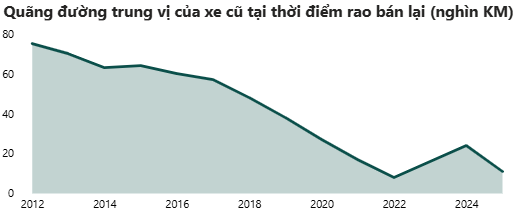
\includegraphics[width=0.8\textwidth]{graphics/Tab04/4.4.PNG}
\caption{Quãng đường trung vị của xe cũ tại thời điểm rao bán lại}
\label{fig:tab4_chart_4_1}
\end{figure}

\noindent\textbf{Loại biểu đồ:} Biểu đồ vùng (area chart).

\begin{itemize}
    \item \textbf{Mục đích và ý nghĩa:} Biểu đồ nhằm theo dõi diễn biến quãng đường trung vị của xe cũ khi được rao bán lại qua từng năm, từ đó suy luận xu hướng nắm giữ hoặc bán lại xe của người dùng đang thay đổi ra sao.

    \item \textbf{Sử dụng dữ liệu:}
    \begin{itemize}
        \item Bảng dữ liệu nguồn: \texttt{fact\_car\_listings}.
        \item Chỉ số: Giá trị trung vị của cột \texttt{Số Km đã đi sạch}.
        \item Cột phân nhóm: \texttt{Năm đăng tin}, trải dài từ 2012 đến 2024.
    \end{itemize}

    \item \textbf{Thiết kế và giải thích:} Dạng biểu đồ vùng giúp nhấn mạnh khối lượng và chiều hướng biến động theo thời gian, phần diện tích tô màu bên dưới đường xu hướng tạo cảm giác trực quan về mức độ suy giảm hay tăng trưởng qua các giai đoạn.

    \item \textbf{Mã hóa trực quan:}
    \begin{itemize}
        \item Trục ngang (X): Năm đăng tin, từ 2012 đến 2024.
        \item Trục dọc (Y): Quãng đường trung vị, đơn vị nghìn km.
        \item Vùng tô màu: Thể hiện giá trị quãng đường trung vị tại mỗi năm, tông xanh nhạt dần khi giá trị giảm.
    \end{itemize}

    \item \textbf{Nhận định và phân tích:}
    \begin{itemize}
        \item Thứ bậc và tỷ trọng chính: Quãng đường trung vị giảm liên tục từ mức khoảng 75 nghìn km năm 2012 xuống mức thấp nhất khoảng 10 nghìn km vào năm 2022, sau đó nhích nhẹ trở lại quanh mốc 20 nghìn km ở các năm gần đây.
        \item Bối cảnh và lý giải: Xu hướng giảm dần cho thấy người dùng có khuynh hướng rao bán lại xe sớm hơn so với trước đây, khi quãng đường đã đi tại thời điểm bán ngày càng thấp, phản ánh chu kỳ nâng đời xe nhanh hơn hoặc tâm lý giữ xe giá trị bán lại cao.
        \item Hạn chế: Đoạn dữ liệu giai đoạn 2022 đến 2023 xuất hiện độ sụt bất thường gần về 0, nhiều khả năng do thiếu dữ liệu hoặc lỗi xử lý outlier, cần rà soát lại trước khi đưa vào kết luận chính thức.
    \end{itemize}
\end{itemize}

\noindent\textbf{Kết luận và đề xuất hành động cho câu hỏi 2:} 
\begin{itemize}
    \item \textbf{Đúc kết cốt lõi:} Hộp số tự động đang dần khẳng định vị thế chủ đạo trên các đời xe sản xuất gần đây, song song với việc quy mô thị trường xe đời mới cũng liên tục mở rộng. Đồng thời, người dùng có xu hướng rao bán lại xe sớm hơn qua từng năm, thể hiện qua quãng đường trung vị giảm dần theo năm sản xuất — cho thấy chu kỳ sở hữu xe đang được rút ngắn. Hai xu hướng này cùng phản ánh một sự dịch chuyển sâu hơn trong thói quen tiêu dùng: người mua xe Việt ngày càng ưu tiên sự tiện dụng tức thời và vòng đời sở hữu ngắn hơn, thay vì gắn bó lâu dài với một chiếc xe như thế hệ trước.
    \item \textbf{Đề xuất hành động:} 
    \begin{itemize}
        \item \textbf{Với đại lý bán lẻ:} Nên ưu tiên nhập các đời xe số tự động cho phân khúc xe đời mới, đồng thời vẫn giữ một tỷ trọng nhỏ xe số sàn cho nhóm khách hàng phổ thông hoặc xe thương mại. Song song đó, cần chú trọng thu mua và tân trang nhóm xe cũ có quãng đường thấp vì đây là nguồn hàng ngày càng phổ biến và dễ bán lại.
        \item \textbf{Với nhóm phân tích:} Nên bổ sung nhãn phần trăm trực tiếp trên đường xu hướng hộp số và tách thêm theo hãng xe để làm rõ hãng nào đang dẫn đầu quá trình chuyển đổi công nghệ truyền động. Đồng thời, có thể đối chiếu quãng đường xe cũ với giá bán để xác nhận liệu xe có quãng đường thấp có thực sự bán được giá tốt hơn hay không.
    \end{itemize}
\end{itemize}
% ------------------------------------------------------------------------------
% 5.X.6 TỔNG KẾT VÀ INSIGHT CHIẾN LƯỢC CẤP TAB
% ------------------------------------------------------------------------------
\subsubsection{Tổng kết và định hướng chiến lược cho tab 4}
\label{subsubsec:tab4_summary}

\noindent\textbf{Tổng hợp các insights chính:}
\begin{itemize}
    \item \textbf{Insight từ câu hỏi 1:} Người mua xe Việt Nam thể hiện sự đồng nhất bất thường trong 2 lựa chọn tưởng chừng mang tính cá nhân — màu ngoại thất và số chỗ ngồi. Nhóm màu trung tính (Trắng, Đen) chiếm tỷ trọng áp đảo so với các màu còn lại, trong khi nhu cầu về cấu hình tập trung chủ yếu vào xe 5 chỗ phục vụ cá nhân và gia đình nhỏ, phân khúc nhiều chỗ chỉ giữ vai trò thứ yếu. Cả hai xu hướng cùng phản ánh một tâm lý tiêu dùng thực dụng: người mua ưu tiên khả năng thanh khoản khi bán lại và chi phí sử dụng hơn là gu thẩm mỹ cá nhân hay quy mô gia đình lớn.
    \item \textbf{Insight từ câu hỏi 2:} Hộp số tự động đang dần thay thế số sàn trên các đời xe sản xuất gần đây, song song với việc quy mô nguồn cung xe đời mới liên tục mở rộng qua từng năm. Đồng thời, quãng đường trung vị của xe cũ tại thời điểm rao bán lại giảm dần theo năm sản xuất, cho thấy người dùng có xu hướng bán lại xe sớm hơn và chu kỳ sở hữu xe đang được rút ngắn. Hai xu hướng này cùng phản ánh một sự dịch chuyển sâu hơn trong thói quen tiêu dùng: người mua xe Việt ngày càng ưu tiên sự tiện dụng tức thời và vòng đời sở hữu ngắn hơn so với thế hệ trước.
\end{itemize}

\noindent\textbf{Trả lời câu hỏi tổng thể:} Chân dung người mua xe Việt Nam hiện nay nghiêng về sự an toàn và thực dụng, ưu tiên màu sắc trung tính dễ bán lại, hộp số tự động tiện dụng, cấu hình 5 chỗ phù hợp nhu cầu cá nhân hoặc gia đình nhỏ, đồng thời có xu hướng nâng đời hoặc thay xe với chu kỳ ngày càng ngắn hơn so với trước đây.

\noindent\textbf{Khuyến nghị và hàm ý thực tiễn:}
\begin{itemize}
    \item \textbf{Đối với doanh nghiệp và nhà quản lý:} Đại lý nên ưu tiên nhập xe màu trung tính, hộp số tự động và cấu hình 5 chỗ vì đây là nhóm có khả năng thanh khoản nhanh nhất, đồng thời chuẩn bị nguồn hàng thu mua xe cũ quãng đường thấp để đáp ứng chu kỳ thay xe ngày càng nhanh của người tiêu dùng.
    \item \textbf{Đối với người mua:} Người mua xe cũ có thể ưu tiên tìm các xe cấu hình phổ biến (màu trung tính, số tự động, 5 chỗ) để dễ dàng bán lại trong tương lai, đồng thời cân nhắc thời điểm bán xe hợp lý để tối ưu giá trị thu hồi trước khi quãng đường sử dụng tăng quá cao.
\end{itemize}

\subsection{Mục tiêu 5: Góc khuất thị trường}
\label{subsec:tab5}

% ------------------------------------------------------------------------------
% 5.5.1 BOI CANH VA MO HINH DU LIEU CUA TAB
% ------------------------------------------------------------------------------
\subsubsection{Bối cảnh phân tích và mô hình dữ liệu}
\label{subsubsec:tab5_schema}

\noindent\textbf{Bối cảnh và mục tiêu phân tích:}
Bốn tab trước xây dựng bức tranh tổng quát về thị trường theo chiều thị phần, giá cả, nhiên liệu và hành vi người mua. Tab 5 tiếp cận từ một góc khác: thay vì mô tả quy luật chung, tab này đi tìm những điểm dữ liệu nằm ngoài quy luật đó. Phân tích tập trung vào ba nhóm câu hỏi: mức giá thực tế ở hai đầu cực của thị trường là bao nhiêu, biên độ dao động giá trong nội bộ một thương hiệu rộng đến đâu, và liệu có hiện tượng đột biến nguồn cung bất thường nào xảy ra theo thời gian. Câu hỏi tổng thể của tab này là: Những điểm dữ liệu bất thường trên thị trường ô tô Việt Nam tiết lộ điều gì về cấu trúc định giá và chuỗi cung ứng?

\begin{table}[H]
\centering
\small
\begin{tabularx}{\textwidth}{L{3cm} L{3.5cm} L{4cm} Y}
\textbf{Tên cột} & \textbf{Bảng nguồn} & \textbf{Ý nghĩa dữ liệu} & \textbf{Phục vụ phân tích} \\ \hline
Giá (triệu VND) & fact\_car\_listings & Mức giá chào bán của phương tiện & Tính giá cực tiểu, cực đại và biên độ chênh lệch nội bộ theo hãng \\
Số km đã đi sạch & fact\_car\_listings & Quãng đường thực tế xe đã lăn bánh & Xác định nhóm xe chạy nhiều km nhất còn được rao bán \\
Năm sản xuất & fact\_car\_listings & Tuổi đời của xe từ 1990 đến 2025 & Trục thời gian phát hiện đột biến nguồn cung theo năm \\
Tên hãng & dim\_brand & Thương hiệu sản xuất & Phân nhóm để đo biên độ dao động giá nội bộ theo hãng \\
\end{tabularx}
\caption{Các trường dữ liệu khai thác cho Tab 5.}
\label{tab:schema_tab5}
\end{table}

% ------------------------------------------------------------------------------
% 5.5.2 KHOI CHI SO KPI TONG QUAN
% ------------------------------------------------------------------------------
\subsubsection{Khối chỉ số KPI tổng quan}
\label{subsubsec:tab5_kpi}


\begin{table}[H]
\centering
\small
\begin{tabularx}{\textwidth}{L{3.5cm} L{2.5cm} L{4cm} Y}
\textbf{Thẻ KPI} & \textbf{Giá trị ghi nhận} & \textbf{Công thức hoặc logic} & \textbf{Ý nghĩa định hướng} \\ \hline
Xe $>$50k km đắt nhất & 12.980 triệu VND & MAX giá của nhóm xe có ODO $>$ 50.000 km & Cho thấy xe siêu sang vẫn giữ giá trị lớn dù cường độ sử dụng cao \\
Xe chạy nhiều km nhất & 500.000 km & MAX của cột số km đã đi sạch & Xác định giới hạn khấu hao vật lý cao nhất được ghi nhận trên hệ thống \\
Số hãng xe hiếm ($\leq$5 xe) & 33 hãng & Đếm số hãng có tổng tin đăng $\leq$ 5 xe & Định lượng nhóm thương hiệu ngách gần như vô hình trên thị trường \\
Lượng xe Ford (SX 2023) & 1.081 xe & Đếm tổng xe Ford có năm sản xuất 2023 & Cảnh báo điểm đột biến nguồn cung bất thường cần xem xét kỹ \\
\end{tabularx}
\caption{Các chỉ số KPI điều hướng trên dashboard Tab 5.}
\label{tab:kpi_tab5}
\end{table}

% ------------------------------------------------------------------------------
% 5.5.3 CAU HOI SMART 1
% ------------------------------------------------------------------------------
\subsubsection{Câu hỏi 1}
\label{subsubsec:tab5_q1}

\noindent \textbf{Nội dung câu hỏi: Mức giá ở hai đầu cực của thị trường được thiết lập như thế nào, và biên độ chênh lệch giá nội bộ của các thương hiệu hạng sang phân bố ra sao?}

\begin{figure}[H]
\centering
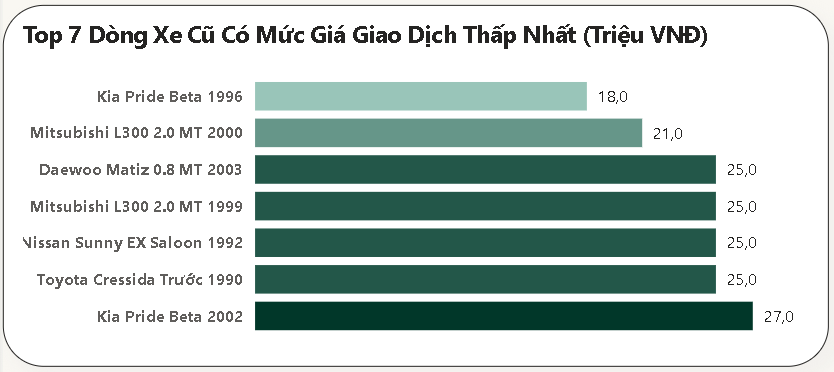
\includegraphics[width=0.95\textwidth]{graphics/Tab05/5.1.PNG}
\caption{Các dòng xe có mức giá thấp nhất thị trường (triệu VND).}
\label{fig:tab5_chart_1}
\end{figure}

\begin{figure}[H]
\centering
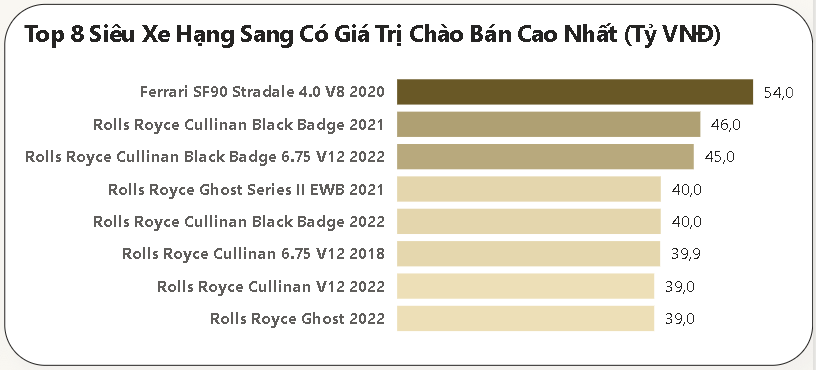
\includegraphics[width=0.95\textwidth]{graphics/Tab05/5.2.PNG}
\caption{Các dòng xe có mức giá cao nhất thị trường (tỷ VND).}
\label{fig:tab5_chart_2}
\end{figure}

\noindent\textbf{Loại biểu đồ:} Biểu đồ thanh ngang, hiển thị hai bảng xếp hạng đặt cạnh nhau.

\begin{itemize}
    \item \textbf{Mục đích và ý nghĩa:} Trực quan hóa đồng thời hai đuôi phân phối giá của thị trường: nhóm xe chạm đáy khấu hao và nhóm xe thiết lập mức giá trần. Đặt hai bảng cạnh nhau giúp khoảng chênh lệch hàng nghìn lần hiện ra ngay lập tức mà không cần thêm chú thích.

    \item \textbf{Sử dụng dữ liệu:}
    \begin{itemize}
        \item Bảng dữ liệu nguồn: \texttt{fact\_car\_listings} kết hợp \texttt{dim\_brand}.
        \item Chỉ số: Cột Giá, lấy theo đơn vị triệu VND ở bảng bên trái và tỷ VND ở bảng bên phải.
        \item Điều kiện lọc: Top 7 dòng xe có giá thấp nhất và Top 8 dòng xe có giá cao nhất.
    \end{itemize}

    \item \textbf{Thiết kế và giải thích:} Biểu đồ thanh ngang được chọn vì tên các phiên bản xe thường dài, cần hiển thị đầy đủ trên nhãn. Hai bảng dùng hai tông màu đối lập, xanh lá cho xe rẻ và nâu vàng cho xe đắt, để phân biệt ngay từ cái nhìn đầu tiên. Thanh được sắp xếp từ giá thấp nhất ở trên, tạo chiều tăng dần từ trên xuống nhất quán ở cả hai bảng.

    \item \textbf{Mã hóa trực quan:}
    \begin{itemize}
        \item Trục ngang (X): Mức giá, đơn vị triệu VND ở bảng bên trái và tỷ VND ở bảng bên phải.
        \item Trục dọc (Y): Tên dòng xe kèm năm sản xuất, sắp xếp tăng dần theo giá từ trên xuống.
        \item Nhãn dữ liệu: Giá trị hiển thị trực tiếp ở cuối mỗi thanh để người đọc không cần gióng sang trục X.
    \end{itemize}

    \item \textbf{Nhận định và phân tích:}
    \begin{itemize}
        \item Đáy thị trường: Mức giá thấp nhất được ghi nhận là 18 triệu VND, thuộc về Kia Pride Beta sản xuất năm 1996. Toàn bộ 7 dòng xe trong danh sách có mức giá từ 18 đến 27 triệu VND, chủ yếu là xe nhỏ và xe tải nhẹ sản xuất trước năm 2005. Đây là nhóm xe đã trải qua hơn hai thập kỷ khấu hao, mức giá thực tế gần như phản ánh giá trị thanh lý phụ tùng hơn là giá trị phương tiện.
        \item Đỉnh thị trường: Ferrari SF90 Stradale 4.0 V8 năm 2020 giữ vị trí cao nhất với 54 tỷ VND, tiếp theo là hai phiên bản Rolls Royce Cullinan Black Badge ở mức 46 và 45 tỷ VND. Đáng chú ý là 7 trong 8 vị trí xe đắt nhất thuộc về Rolls Royce, với các phiên bản dao động từ 39 đến 46 tỷ VND. Lamborghini và Bentley, hai thương hiệu thường được liên tưởng đến mức giá đỉnh, không có mặt trong Top 8 này.
        \item So sánh tổng thể: Khoảng cách giữa chiếc xe rẻ nhất (18 triệu VND) và đắt nhất (54 tỷ VND) lên tới hơn 3.000 lần. Cả hai cùng tồn tại trên một nền tảng rao bán, trong cùng một bộ dữ liệu, phản ánh tính đa dạng cực đoan của hàng hóa ô tô so với hầu hết các loại tài sản tiêu dùng khác.
    \end{itemize}
\end{itemize}

\begin{figure}[H]
\centering
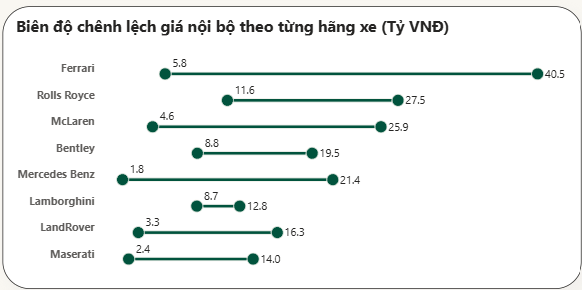
\includegraphics[width=0.95\textwidth]{graphics/Tab05/5.3_Dumbbell.png}
\caption{Biên độ chênh lệch giá nội bộ theo từng hãng xe hạng sang (tỷ VND).}
\label{fig:tab5_chart_3}
\end{figure}

\noindent\textbf{Loại biểu đồ:} Biểu đồ quả tạ.

\begin{itemize}
    \item \textbf{Mục đích và ý nghĩa:} Đo lường biên độ dao động giá trong nội bộ mỗi thương hiệu, trả lời câu hỏi liệu cùng một thương hiệu có thể bán xe ở những mức giá khác nhau đến đâu. Biểu đồ này không hỏi hãng nào đắt hay rẻ mà hỏi hãng nào có khoảng phân tán nội bộ lớn nhất.

    \item \textbf{Sử dụng dữ liệu:}
    \begin{itemize}
        \item Bảng dữ liệu nguồn: \texttt{fact\_car\_listings} kết hợp \texttt{dim\_brand}.
        \item Chỉ số: Với mỗi hãng, tính hai giá trị là biên độ xuống (\texttt{Median} $-$ \texttt{Min}) và biên độ lên (\texttt{Max} $-$ \texttt{Median}), đơn vị tỷ VND.
        \item Điều kiện lọc: Top 8 hãng có tổng biên độ (\texttt{Max} $-$ \texttt{Min}) lớn nhất.
    \end{itemize}

    \item \textbf{Thiết kế và giải thích:} Biểu đồ quả tạ tối ưu tỷ lệ data-ink bằng cách loại bỏ các cột khối nặng nề, chỉ dùng đường nối và hai điểm đầu cuối để truyền tải thông tin về khoảng cách. Điểm bên trái thể hiện biên độ xuống phía giá thấp, điểm bên phải thể hiện biên độ lên phía giá cao. Cách biểu diễn này giúp người đọc so sánh cả độ rộng lẫn vị trí tương đối của mỗi hãng chỉ trong một lượt quan sát.

    \item \textbf{Mã hóa trực quan:}
    \begin{itemize}
        \item Trục ngang (X): Biên độ giá, đơn vị tỷ VND.
        \item Trục dọc (Y): Tên hãng xe, sắp xếp từ tổng biên độ lớn nhất ở trên xuống nhỏ nhất ở dưới.
        \item Điểm marker: Cả hai điểm đầu cuối đều dùng màu xanh đậm. Điểm bên trái thể hiện biên độ xuống (median $-$ min), điểm bên phải thể hiện biên độ lên (max $-$ median). Đường nối màu xanh nhạt hơn thể hiện tổng khoảng phân tán.
        \item Nhãn dữ liệu: Giá trị số ghi trực tiếp cạnh mỗi điểm marker.
    \end{itemize}

    \item \textbf{Nhận định và phân tích:}
    \begin{itemize}
        \item Biên độ lớn nhất: Ferrari dẫn đầu với tổng biên độ 46,3 tỷ VND, trong đó biên độ xuống là 5,8 tỷ và biên độ lên là 40,5 tỷ. Cấu trúc lệch mạnh về phía biên độ lên cho thấy phần lớn xe Ferrari trong dữ liệu tập trung ở vùng giá thấp hơn, trong khi chỉ một số ít phiên bản đẩy trần lên rất cao. Rolls Royce xếp thứ hai với tổng biên độ 39,1 tỷ VND, biên độ xuống 11,6 tỷ và biên độ lên 27,5 tỷ. McLaren đứng thứ ba với tổng biên độ 30,5 tỷ (4,6 và 25,9), tiếp theo là Bentley với 28,3 tỷ (8,8 và 19,5).
        \item Trường hợp đặc biệt của Mercedes Benz: Mercedes có biên độ xuống chỉ 1,8 tỷ VND nhưng biên độ lên tới 21,4 tỷ VND, tổng biên độ 23,2 tỷ. Cấu trúc lệch mạnh này cho thấy giá trung vị của Mercedes nằm rất gần với mức giá thấp nhất của hãng trong dữ liệu, tức phần lớn xe Mercedes thuộc phân khúc tầm trung, trong khi chỉ một nhóm nhỏ phiên bản hiệu năng cao đẩy giá trần lên rất xa so với mặt bằng chung.
        \item Ba hãng còn lại: Lamborghini (8,7 và 12,8, tổng 21,5 tỷ), LandRover (3,3 và 16,3, tổng 19,6 tỷ) và Maserati (2,4 và 14,0, tổng 16,4 tỷ) có tổng biên độ thấp hơn so với nhóm đầu nhưng vẫn phản ánh mức phân tán đáng kể trong nội bộ mỗi hãng. Thứ tự trên biểu đồ phản ánh tổng biên độ tuyệt đối, không phản ánh độ phổ biến hay quy mô thị phần.
    \end{itemize}
\end{itemize}

\noindent\textbf{Kết luận và đề xuất hành động cho câu hỏi 1:}
\begin{itemize}
    \item \textbf{Đúc kết cốt lõi:} Thị trường tồn tại khoảng cách định giá lên tới hơn 3.000 lần giữa xe rẻ nhất và đắt nhất. Thương hiệu không đại diện cho một mức giá cố định mà bao hàm một khoảng phân tán rộng, đặc biệt với nhóm xe hạng sang, nơi mỗi phiên bản và tình trạng xe có thể tạo ra mức giá chênh lệch hàng chục tỷ đồng.
    \item \textbf{Đề xuất hành động:}
    \begin{itemize}
        \item \textbf{Với hệ thống gợi ý sản phẩm:} Khi phân cụm dữ liệu theo khoảng giá, cần phân cụm theo phiên bản và cấu hình cụ thể thay vì gom theo thương hiệu, để tránh gợi ý lệch cho người dùng khi cùng một hãng có thể bán xe ở những mức giá cách nhau vài chục tỷ đồng.
        \item \textbf{Với người mua xe hạng sang:} Cần so sánh kỹ theo phiên bản và năm sản xuất, không nên dùng tên thương hiệu như một đại diện cho mức giá tham chiếu.
    \end{itemize}
\end{itemize}

% ------------------------------------------------------------------------------
% 5.5.4 CAU HOI SMART 2
% ------------------------------------------------------------------------------
\subsubsection{Câu hỏi 2}
\label{subsubsec:tab5_q2}

\noindent \textbf{Nội dung câu hỏi: Có hiện tượng đột biến nguồn cung bất thường nào theo năm sản xuất ở các thương hiệu phổ thông không?}

\begin{figure}[H]
\centering
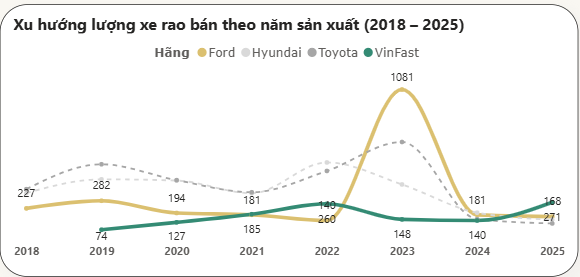
\includegraphics[width=0.95\textwidth]{graphics/Tab05/5.4_LineChart.png}
\caption{Xu hướng lượng xe rao bán theo năm sản xuất của bốn hãng lớn (2018--2025).}
\label{fig:tab5_chart_4}
\end{figure}

\noindent\textbf{Loại biểu đồ:} Biểu đồ đường nhiều chuỗi.

\begin{itemize}
    \item \textbf{Mục đích và ý nghĩa:} Theo dõi diễn biến số lượng xe rao bán theo năm sản xuất của từng hãng, phát hiện các năm có lượng xe đột biến so với xu hướng chung. Biểu đồ này không hỏi tổng số xe là bao nhiêu mà hỏi liệu có hãng nào xuất hiện bất thường tại một thời điểm cụ thể không.

    \item \textbf{Sử dụng dữ liệu:}
    \begin{itemize}
        \item Bảng dữ liệu nguồn: \texttt{fact\_car\_listings} kết hợp \texttt{dim\_brand}.
        \item Trục ngang (X): Năm sản xuất, từ 2018 đến 2025.
        \item Trục dọc (Y): Số lượng xe rao bán, đếm theo số tin đăng.
        \item Chuỗi dữ liệu: Bốn hãng Ford, Hyundai, Toyota và VinFast, được chọn vì có số lượng xe đáng kể và tạo ra các xu hướng đủ để so sánh.
    \end{itemize}

    \item \textbf{Thiết kế và giải thích:} Biểu đồ đường phù hợp nhất để quan sát dữ liệu theo chuỗi thời gian vì nó làm rõ hướng di chuyển và điểm gãy của từng chuỗi. Bốn đường được gán màu khác nhau, trong đó đường Ford màu vàng nổi bật nhất vì đây là chuỗi chứa điểm đột biến cần chú ý. Nhãn số gắn trực tiếp lên từng điểm dữ liệu để người đọc không cần gióng sang trục Y.

    \item \textbf{Mã hóa trực quan:}
    \begin{itemize}
        \item Trục ngang (X): Năm sản xuất 2018 đến 2025, tăng dần từ trái sang phải.
        \item Trục dọc (Y): Số lượng xe, đơn vị chiếc.
        \item Màu sắc: Mỗi hãng một màu riêng biệt, đường Ford màu vàng được phân biệt rõ với ba đường còn lại.
        \item Nhãn dữ liệu: Số lượng cụ thể hiển thị tại mỗi điểm năm trên tất cả các đường.
    \end{itemize}

    \item \textbf{Nhận định và phân tích:}
    \begin{itemize}
        \item Điểm bất thường của Ford năm 2023: Trong khi Hyundai, Toyota và VinFast duy trì lượng xe dao động từ 74 đến 704 chiếc mỗi năm theo xu hướng tương đối ổn định, Ford đột ngột đạt 1.081 chiếc ở nhóm xe sản xuất năm 2023, gấp gần 7,7 lần so với mức 140 chiếc của năm 2022. Đây là mức đột biến lớn nhất trong toàn bộ dữ liệu khi nhìn theo chiều hãng và năm sản xuất.
        \item Trước và sau điểm đột biến: Ford đi vào năm 2023 từ mức 140 chiếc năm 2022 và trở về 181 chiếc năm 2024. Không có chuỗi tăng trưởng dẫn trước để giải thích đỉnh 1.081, cũng không có chuỗi giảm dần sau đó. Đây là dạng đột biến cục bộ, không phải xu hướng kéo dài.
        \item Khả năng lý giải: Dữ liệu không đủ để kết luận nguyên nhân chính xác. Một số khả năng có thể xem xét là lô xe thương mại hoặc xe dịch vụ hết hạn hợp đồng được xả ra cùng lúc, hoặc lô xe lái thử từ hệ thống đại lý được thanh lý đồng loạt. Điều quan trọng là chính việc dữ liệu không tự giải thích được điểm bất thường này là một tín hiệu cần chú ý trong quá trình xây dựng mô hình.
        \item VinFast năm 2025: VinFast đạt 271 chiếc ở nhóm xe sản xuất năm 2025, vượt qua cả Toyota (119 chiếc), Hyundai (146 chiếc) và Ford (168 chiếc) trong cùng năm. Đây là lần đầu tiên VinFast dẫn đầu về số lượng trong nhóm xe đời mới nhất, kết quả nhất quán với xu hướng tăng trưởng thị phần xe điện đã được ghi nhận tại Tab 3.
    \end{itemize}
\end{itemize}

\noindent\textbf{Kết luận và đề xuất hành động cho câu hỏi 2:}
\begin{itemize}
    \item \textbf{Đúc kết cốt lõi:} Nguồn cung trên thị trường không phân phối đồng đều theo thời gian. Trường hợp Ford năm 2023 với 1.081 chiếc là một điểm đột biến cục bộ rõ ràng, không phải xu hướng ổn định. Nếu đưa điểm này vào mô hình học máy mà không xử lý riêng, hệ thống có thể học nhầm phân phối bất thường này là quy luật chung của thị trường Ford.
    \item \textbf{Đề xuất hành động:}
    \begin{itemize}
        \item \textbf{Với nhóm xây dựng mô hình:} Cần gán nhãn và tách riêng tập dữ liệu Ford năm 2023 trước khi huấn luyện bất kỳ mô hình nào liên quan đến dự báo cung hoặc định giá, để tránh mô hình bị ảnh hưởng quá mức bởi một điểm bất thường không đại diện cho xu hướng thực.
        \item \textbf{Với nhóm phân tích:} Nên bổ sung dữ liệu ngoài (ví dụ thông tin từ các đại lý Ford hoặc báo cáo doanh số ngành) để xác minh nguồn gốc của đỉnh 1.081 xe trước khi đưa ra kết luận chính thức.
    \end{itemize}
\end{itemize}

% ------------------------------------------------------------------------------
% 5.5.5 TONG KET VA INSIGHT CHIEN LUOC CAP TAB
% ------------------------------------------------------------------------------
\subsubsection{Tổng kết và định hướng chiến lược cho tab 5}
\label{subsubsec:tab5_summary}

\noindent\textbf{Tổng hợp các Insights chính:}
\begin{itemize}
    \item \textbf{Insight từ câu hỏi 1:} Thị trường có khoảng cách định giá lên tới hơn 3.000 lần giữa xe rẻ nhất (18 triệu VND) và đắt nhất (54 tỷ VND). Các thương hiệu hạng sang có biên độ dao động giá nội bộ rất lớn, trong đó Ferrari dẫn đầu với tổng biên độ 46,3 tỷ VND. Thương hiệu không tương đương với một mức giá cụ thể mà bao hàm một dải phân tán rộng phụ thuộc vào phiên bản và tình trạng xe.
    \item \textbf{Insight từ câu hỏi 2:} Ford sản xuất năm 2023 xuất hiện với 1.081 chiếc, gấp 7,7 lần so với năm trước và trở về mức bình thường ngay sau đó. Đây là điểm bất thường cục bộ về nguồn cung không có giải thích rõ ràng từ dữ liệu. VinFast lần đầu dẫn đầu số lượng xe đời mới năm 2025 với 271 chiếc, vượt qua cả Toyota, Hyundai và Ford trong cùng nhóm năm sản xuất.
\end{itemize}

\noindent\textbf{Trả lời câu hỏi tổng thể:} Thị trường ô tô Việt Nam chứa đựng những điểm dữ liệu bất thường ở cả hai chiều: chiều giá trị tài sản với khoảng phân tán hàng chục tỷ đồng trong cùng một thương hiệu, và chiều cung ứng với các đợt xả hàng đột biến không theo quy luật tăng trưởng thông thường. Những điểm bất thường này không phải nhiễu cần loại bỏ mà là tín hiệu cần được xử lý có chủ đích trước khi đưa dữ liệu vào các bước phân tích tiếp theo.

\noindent\textbf{Khuyến nghị và hàm ý thực tiễn:}
\begin{itemize}
    \item \textbf{Đối với doanh nghiệp và nhà quản lý nền tảng:} Cần thiết lập bộ lọc động để cô lập các tin đăng rơi vào vùng giá cực đoan, tránh làm lệch các báo cáo thống kê trung bình cung cấp cho người dùng phổ thông. Một chiếc xe 54 tỷ đồng nếu được tính vào giá trung vị chung sẽ kéo lệch đáng kể so với thực tế mà đa số người mua tiếp cận.
    \item \textbf{Đối với nhóm xây dựng mô hình dữ liệu:} Trước khi đưa tập dữ liệu này vào huấn luyện hệ thống gợi ý hoặc mô hình dự báo giá, cần xử lý riêng hai nhóm: nhóm xe có giá nằm ngoài khoảng phân vị thứ 5 đến thứ 95 để chuẩn hóa thang đo giá, và nhóm xe Ford năm 2023 để tránh mô hình học nhằm phân phối đột biến không đại diện cho xu hướng thực.
\end{itemize}

\clearpage